\chapter{Feature-based Regularizations}
\label{chapter:regularization}

%\newcommand{\mcL}{\mathcal{L}} \newcommand{\vx}{\mathbf{x}} \newcommand{\vh}{\mathbf{h}}
%\newcommand{\vy}{\mathbf{y}}
\newcommand{\tableindent}{\,\,\,\,}
\newcommand{\vt}{\mathbf{t}}
%\newcommand{\vyh}{\hat\vy}
\newcommand{\std}{$\pm\,$}
\newcommand{\clf}{\textit{clf}} \newcommand{\gray}[1]{{\color{darkgray}#1}}


\begin{chapabstract}
    Regularization-based methods are powerful approaches to reduce catastrophic forgetting,
    especially in challenging setting such as \ac{CIL} with single-head where task identity is not
    known at test-time. However, they often consider only constraining the final probability
    predictions of the network, weakly constraining the model's behavior and in turns falls short to
    forgetting when faced to large amount of tasks. \\
    In this chapter, we propose two methods exploiting explicitly the intermediate features to
    reduce forgetting. The first approach, nicknamed PODNet, aims to constrain similar statistics to
    avoid a representation drift at all levels of the network. We show that it scales particularly
    well on extreme scenarios where classes are learned one by one for a long succession of
    iterations, due to its balancing of rigidity (not forgetting old classes) - plasticity (learning
    new classes) tradeoff. The second approach, named Ghost, pre-emptively reserves capacity for
    future ---yet to be seen--- classes avoiding forgetting before it even happens. We pinpoint
    those classes locations in the representation space by estimating their future positions by
    drawing inspiration from the \ac{ZSL} literature using their metadata.

    The work in this section has led to a publication to two papers:

    \begin{itemize}
        \item \fullcite{douillard2020podnet}
        \item \fullcite{douillard2020ghost}
    \end{itemize}

\end{chapabstract}
\newpage

\minitoc
\chapterwithfigures{\nameref*{chapter:regularization}}
\chapterwithtables{\nameref*{chapter:regularization}}

\ifthenelse{\boolean{skipRegul}}{\endinput}{}

\section{Introduction}

\acf{CIL}, where each task brings new classes, is among the most challenging setting of \acf{CL}. When
evaluated in single-head, where the task identity is not known at test-time, the majority of the
methods rely on rehearsal learning where a limited amount of old data is replayed. Furthermore, it
is often combined to regularizations that aim to limit forgetting. These regularizations are often a
knowledge distillation \citep{hinton2015knowledge_distillation} that enforces similar probabilities
between the old and current model. First introduced by LwF \citep{li2018lwf}, it has be used
afterwards by multiple seminal papers including iCaRL \citep{rebuffi2017icarl} and WA
\citep{zhao2020weightalignement}. We propose in this chapter two proposed regularization methods to
reduce forgetting. The first one, introduced in \acf{PODNet} \citep{douillard2020podnet} and detailed
in \autoref{sec:podnet}, aims to regularize the statistics shift at the intermediate feature-level
to enforce a consistent representation at multiple levels of the feature extractor across all steps
of the continual training. The second one, nicknamed Ghost \citep{douillard2020ghost} and described
in \autoref{sec:ghost}, on the other hand, avoid pre-emptively forgetting by regularizing the
feature space at locations where the model estimates future classes will be.

For both PODNet and Ghost, we will focus on \ac{CIL} where each new task brings new classes. We
propose then to split a dataset into multiple tasks, \eg CIFAR100 50-1 would be 1 task of 50 classes
followed by 50 tasks of 1 class each. Following other output-based regularization methods
(\autoref{sec:related_regul_output}), we allow a rehearsal memory storing a limited amount of
previous data (\autoref{sec:related_rehearsal}).

\section{PODNet: reducing forgetting via intermediate feature statistics}
\label{sec:podnet}

\subsection{Related Works}
\label{sec:podnet_related}

We frame our model onto two paradigms: representation learning and regularization-based.

\paragraph{Regularization of the model's output} Regularizations constraining the rate of change of
the weights \citep{kirkpatrick2017ewc} or the gradients \citep{farajtabar2020ogd} have been
proposed. They reduce effectively the forgetting of the feature extractors in a multi-heads setting
where the task identity is known at test-time. However, in the more challenging and realist setting
of single-head, where classes from all tasks, have to be predicted, these methods often barely work
better than a naive finetuning \citep{lesort2019regulshortcomings}. Therefore, We focused on
regularizations applied on a model's output. LwF \citep{li2018lwf} first used the \ac{KD} of
\cite{hinton2015knowledge_distillation}: a KL divergence between the probabilities of the old and
new models. While simple, this loss ---with few variations--- has been used by multiple following
works \citep{rebuffi2017icarl,zhao2020weightalignement}. Few works tried to constrain intermediate
outputs of the model: LwM \citep{dhar2019learning_without_memorizing_gradcam} proposed to minimize
the L2 distance between gradient-based attention maps produced by GradCam
\citep{selvaraju2017gradcam}. M2KD \citep{peng2019m2kd} used a \ac{KD} on both the final predictions
and intermediate predictions from an auxiliary classifier similar to Inception
\citep{szegedy2015inception}. \cite{hou2019ucir} maximizes the cosine similarity between the final
embeddings before the classifier. Finally, \cite{zagoruyko2016distillation_attention}, in the
context of model compression, investigated attention-based distillation for image classifiers, by
pooling the intermediate features of convolutional networks into attention maps, then used in their
distillation losses.

\paragraph{Representation learning} was already implicitly present in
iCaRL~\citep{rebuffi2017icarl}: it introduced the \acf{NME} strategy which
averages the outputs of the deep convolutional network to create a single proxy feature vector per
class that are then used by a nearest-neighbor classifier predict the final classes.
\cite{hou2019ucir} adopted this method and also introduced another, named CNN, which uses the output
class probabilities to classify incoming samples, freezing (during training) the classifier weights
associated with old classes, and then fine-tuning them on an under-sampled dataset.
\cite{hou2019ucir}, in the method called here UCIR, made representation learning explicit, by
noticing that the limited memory imposed a severe imbalance on the training samples available for
the old and for the new classes. To overcome that difficulty, they designed a metric-learning model
instead of a classification model. That strategy is often used in few-shot
learning~\citep{gidaris2018fewshot_wo_forgetting} because of its robustness when faced to few data. Because
classical metric architectures require special training sampling (\eg semi-hard sampling for
triplets), \cite{luo2018cosine_classifier} chose instead to redesign the classifier's last layer of their model to use
the cosine similarity.


\begin{figure}[tb]
    \begin{center}
        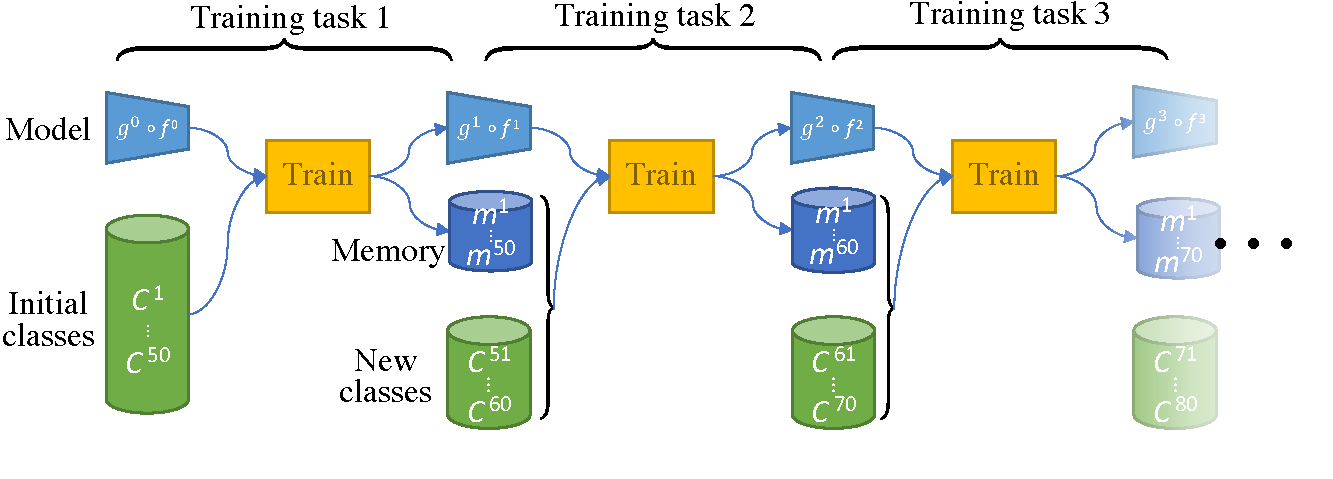
\includegraphics[width=1.0\linewidth]{images/podnet/protocol}
    \end{center}
    \caption{\textbf{Training protocol for incremental learning}. At each training task we learn a
        new set of classes, and the model must retain knowledge about \textit{all} classes. The
        model is allowed a \textit{limited} memory of samples of old classes. In our experiments, the first task
        contain more classes than the following tasks (50 \vs 10 on this figure).}
    \label{fig:podnet_protocol}
\end{figure}

\subsection{Model}
\label{sec:podnet_model}

We follow the notations defined in the \hyperref[chap:notations]{Notations}. Our model is
evaluated in the class incremental setting with rehearsal memory (\autoref{sec:related_rehearsal})
depicted \autoref{fig:podnet_protocol}. Our strategy is made of two keys components: a distillation
loss applied at the intermediate feature-level, and a local-similarity classifier.

\subsubsection{POD: Pooled Outputs Distillation loss}
\label{sec:podnet_pod}

Constraining the evolution of the weights is crucial to reduce forgetting. Each new task $t$ learns
a new (student) model, whose weights are not only initialized with those of the previous (teacher)
model, but also constrained by a distillation loss. That loss must be carefully balanced to prevent
forgetting (rigidity), while allowing the learning of new classes (plasticity).

To this goal, we propose a set of constraints we call \textbf{Pooled Outputs Distillation (POD)},
applied not only over the final embedding output by $\vh^{t}=f^{t}(\vx)$, but also over the output
of its intermediate layers $\vh^{t}_\ell=f^{t}_\ell(\vx)$ (where by notation overloading
$f^{t}_\ell(\vx)\equiv f^{t}_\ell\circ\ldots\circ f^{t}_1(\vx)$, and thus $f^{t}(\vx)\equiv
    f^{t}_L\ldots\circ f^{t}_\ell\circ\ldots f^{t}_1(\vx)$).

The convolutional layers of the network output tensors $\vh^{t}_{\ell}$ with components
$\vh^{t}_\ell[c,w,h]$, where $c$ stands for channel (filter), and $w\times h$ for column and row of
the spatial coordinates. The loss used by POD may pool (sum over) one or several of those indexes,
more aggressive poolings (\autoref{fig:podnet_pooling}) providing more freedom, and thus,
plasticity: the lowest possible plasticity imposes an exact similarity between the previous and
current model while higher plasticity relaxes the similarity definition.

Pooling is an important operation in Computer Vision, with a strong theoretical motivation. In the
past, pooling has been introduced to obtain invariant
representations~\citep{lowe1999sift,lazbnik2006spatial_pyramid_matching}. Here, the justification is
similar, but the goal is different: as we will see, the pooled indexes are aggregated in the
proposed loss, allowing \textit{plasticity}. Instead of the model acquiring invariance to the input
image, the desired loss acquires invariance to model evolution, and thus, representation.
%
The proposed pooling-based formalism has two advantages: first, it organizes disparately proposed
distillation losses into a neat, general formalism. Second, as we will see, it allowed us to propose
novel distillation losses, with better plasticity-rigidity compromises. Those topics are explored
next.

\begin{figure}[tb]
    \begin{center}
        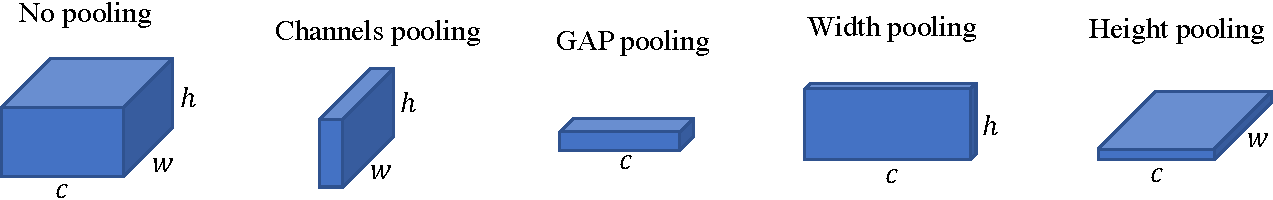
\includegraphics[width=0.90\linewidth]{images/podnet/pooling}
    \end{center}
    \caption{\textbf{Different possible poolings}. The output from a convolutional layer
        $\vh^{t}_\ell[c,w,h]$ may be pooled (summed over) one or more axes. The resulting loss
        considers only the pooled activations instead of the individual components, allowing more
        plasticity across the pooled axes.}
    \label{fig:podnet_pooling}
\end{figure}

\paragraph{Pooling of convolutional outputs} As explained before, POD constrains the output of each
intermediate convolutional layer $\vh^{t}_\ell = f^{t}_\ell(\cdot)$ (in practice, each stage of a
ResNet~\citep{he2016resnet}). All POD variants use the Euclidean distance of $\ell^2$-normalize
tensors, here noted as $\left\Vert\cdot-\cdot\right\Vert$. They differ on the type of pooling
applied before that distance is computed.
%
On one extreme, one can apply no pooling at all, resulting in the most strict loss, the most rigid
constrains, and the lowest plasticity:
%
\begin{equation}
    \mcL_{\text{POD-pixel}}(\vh^{t-1}_\ell, \vh^t_\ell) = \sum_{c=1}^C \sum_{w=1}^{W} \sum_{h=1}^{H} \left\Vert \vh^{t-1}_\ell[c,w,h] - \vh^t_\ell[c,w,h] \right\Vert^2\,.
    \label{eq:podnet_pod_pixel}
\end{equation}
%
By pooling the channels, one preserves only the spatial coordinates, resulting in a more permissive
loss, allowing the activations to reorganize across the channels, but penalizing global changes of
those activations across the space,
%
\begin{equation}
    \mcL_{\text{POD-channel}}(\vh^{t-1}_\ell, \vh^t_\ell)  = \sum_{w=1}^{W} \sum_{h=1}^{H} \left\Vert \sum_{c=1}^C \vh^{t-1}_\ell[c,w,h] - \sum_{c=1}^C \vh^{t}_\ell[c,w,h] \right\Vert^2\,;
    \label{eq:podnet_pod_channel}
\end{equation}
%
\noindent or, contrarily, by pooling the space (equivalent, up to a factor, to a Global Average Pooling), one
preserves \textit{only} the channels:
%
\begin{equation}
    \mcL_{\text{POD-gap}}(\vh^{t-1}_\ell, \vh^t_\ell) = \sum_{c=1}^{C} \left\Vert \sum_{w=1}^{W} \sum_{h=1}^H \vh^{t-1}_\ell[c,w,h] - \sum_{w=1}^{W} \sum_{h=1}^H \vh^{t}_\ell[c,w,h] \right\Vert^2\,.
    \label{eq:podnet_pod_gap}
\end{equation}
%
Note that the only difference between the variants is in the position of the summation. For example,
contrast equations \autoref{eq:podnet_pod_pixel} and \ref{eq:podnet_pod_channel}: in the former the
differences are computed between activation pixels, and then totaled; in the latter, first the
channel axis is flattened, then the differences are computed, resulting in a more permissive loss.

We can trade a little plasticity for rigidity, with less aggressive pooling by aggregating
statistics across just one of the spatial dimensions:
%
\begin{equation}
    \mcL_{\text{POD-width}}(\vh^{t-1}_\ell, \vh^t_\ell)  = \sum_{c=1}^{C} \sum_{h=1}^{H} \left\Vert \sum_{w=1}^W \vh^{t-1}_\ell[c,w,h] - \sum_{w=1}^W \vh^{t}_\ell[c,w,h] \right\Vert^2\,;
    \label{eq:podnet_pod_width}
\end{equation}
%
\noindent or, likewise, for the vertical dimension, resulting in POD-height. Each of those variants measure
the distribution of activation pixels across their respective axis. These two complementary
intermediate statistics can be further combined:
%
\begin{equation}
    \mcL_{\text{POD-spatial}}(\vh^{t-1}_\ell, \vh^t_\ell) = \mcL_{\text{POD-width}}(\vh^{t-1}_\ell, \vh^t_\ell) + \mcL_{\text{POD-height}}(\vh^{t-1}_\ell, \vh^t_\ell)\,.
    \label{eq:podnet_pod_spatial}
\end{equation}
%
$\mcL_{\text{POD-spatial}}$ is minimal when the average statistics over the dataset, on both width
and height axes, are similar for the previous and current model. It brings the right balance between
being too rigid (\autoref{eq:podnet_pod_pixel}) and being too permissive
(\autoref{eq:podnet_pod_channel} and \ref{eq:podnet_pod_gap}).

\label{sec:podnet_pod_flat}
\paragraph{Constraining the final embedding} After the convolutional layers, the network, by design,
flattens the spatial coordinates, and the formalism above needs adjustment, as a summation over $w$
and $h$ is no longer possible. Instead, we set a flat constraint on the final embedding $\vh^{t} =
    f^{t}(\vx)$:
%
\begin{equation}
    \mcL_{\text{POD-flat}}(\vh^{t-1}, \vh^t) = \left\Vert \vh^{t-1} - \vh^t \right\Vert^2\,.
    \label{eq:podnet_pod_flat}
\end{equation}

\paragraph{Combining the losses, analysis} The final POD loss combines the two  components:
%
\begin{multline}
    \mcL_\text{POD-final}(\vx) =  \frac{\lambda_{c}}{L-1}\sum_{\ell=1}^{L-1}  \mcL_{\text{POD-spatial}}\left(f^{t-1}_\ell(\vx), f^t_\ell(\vx)\right) + \\[-0.8em]
    \lambda_{f} \mcL_\text{POD-flat}\left(f^{t-1}(\vx), f^t(\vx)\right)\,.
    \label{eq:podnet_pod_final}
\end{multline}
%
The hyperparameters $\lambda_{c}$ and $\lambda_{f}$ are necessary to balance the two terms, due to
the different nature of the intermediate outputs (spatial and flat).

As mentioned, the strategy above generalizes disparate propositions existing both in the literature
of incremental learning, and elsewhere. When $\lambda_{c}=0$, it reduces to the cosine constraint of
\textit{Less-Forget}, proposed by \cite{hou2019ucir} for incremental learning, which constrains only
the final embedding. When $\lambda_{f}=0$ and POD-spatial is replaced by POD-pixel, it suggests the
Perceptual Features loss, proposed for style transfer~\citep{johnson2016perceptual_losses}. When
$\lambda_{f}=0$ and POD-spatial is replaced by POD-channel, the strategy hints at the loss proposed
by \cite{zagoruyko2016distillation_attention} to allow distillation across different networks, a
situation in which the channel pooling responds to the very practical need to allow the comparison
of architectures with different number of channels.

As we will see in our evaluations of pooling strategies (\autoref{sec:podnet_ablation_pooling}),
what proved optimal was a completely novel idea, POD-spatial, combining two poolings, each of which
flattens one of the spatial coordinates. That relatively rigid strategy (channels and one of the
spatial coordinates are considered in each half of the loss) makes intuitive sense in our context,
which is \textit{small-task} incremental learning, and thus where we expect a slow drift of the
model across a single task.

% ------------------------------------------------------------

\begin{figure}[t]
    \begin{center}
        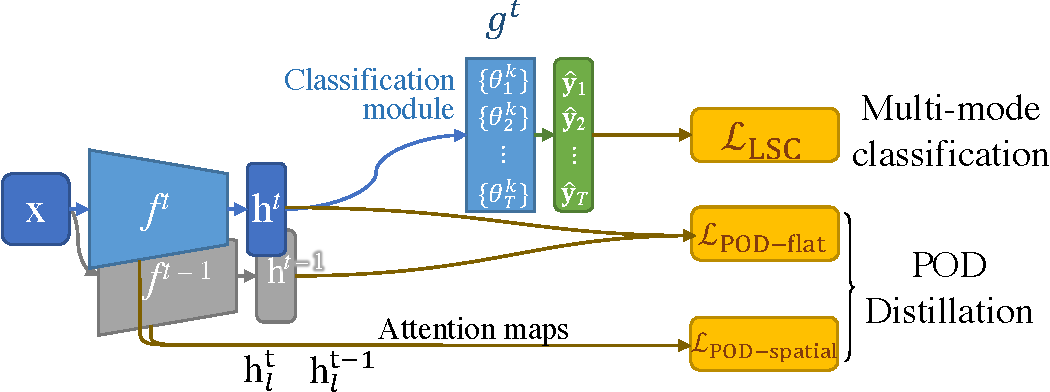
\includegraphics[width=0.8\linewidth]{images/podnet/model}
    \end{center}
    \caption{\textbf{Overview of PODNet}: the distillation loss \ac{POD} prevent excessive model
        drift by constraining intermediate outputs of the \ac{ConvNet} $f$ and the \ac{LSC}
        classifier $g$ learns a more expressive multi-modal representation.}
    \label{fig:podnet_model}
\end{figure}

\subsubsection{Local Similarity Classifier}
\label{sec:podnet_local_classifier}

\cite{hou2019ucir} observed that the class imbalance of incremental learning has concrete
manifestations on the parameters of the final layer on classifiers, namely the weights for the
over-represented (new) classes becoming much larger than those for the underrepresented (old)
classes. To overcome this issue, their method (called here UCIR) $\ell^2$-normalizes both the
weights and the activations, which corresponds to taking the cosine similarity instead of the dot
product. For each class $c$, their last layer becomes
%
\begin{equation}
    \vyh_{c}=\frac{\exp\left(\eta\langle\theta_{c},\vh\rangle\right)}{\sum_{i} \exp \left(\eta\langle\theta_{i}, \vh\rangle\right)}\,,
\end{equation}
%
\noindent where $\theta_c$ are the last-layer weights for class $c$, $\eta$ is a learned scaling parameter,
and $\langle\cdot,\cdot\rangle$ is the cosine similarity.

However, this strategy optimizes a \textit{global similarity}: its training objective increases the
similarity between the extracted features and their associated weights. For each class, the
normalized weight vector acts as a \textit{single} proxy~\citep{attias2017proxynca}, towards which
the learning procedure pushes all samples in the class.

We observed that such global strategy is hard to optimize in an incremental setting. To avoid
forgetting, the distillation losses (\autoref{sec:podnet_pod}) tries to keep the final embedding
$\vh$ consistent through time so that the class proxies stay relevant for the classifier.
Unfortunately catastrophic forgetting, while alleviated by current methods, is not solved and thus
the distribution of $\vh$ may change. The cosine classifier is very sensitive to those changes as it
models a unique majority mode through its class proxies.


\paragraph{Local Similarity Classifier} The problem above lead us to amend the classification layer
during training, in order to consider multiple proxies/modes per class. A shift in the distribution
of $\vh$ will have less impact on the classifier as more modes are covered.


Our redesigned classification layer, which we call Local Similarity Classifier (LSC), allows for $K$
multiple proxies/modes during training. Like before, the proxies are a way to interpret the weight
vector in the cosine similarity, thus we allow for $K$ vectors $\theta_{c,k}$ for each class $c$.
The similarity $s_{c,k}$ to each proxy/mode is first computed. An averaged class similarity $\vyh_c$
is the output of the classification layer:
%
\begin{equation}
    s_{c,k} =\frac{\exp\,\langle\theta_{c,k},\vh\rangle}{\sum_{i} \exp\,\langle\theta_{c,i},\vh\rangle}\,, \qquad
    \vyh_c = \sum_{k}s_{c,k}\,\langle\theta_{c,k},\vh\rangle\,.
    \label{eq:podnet_lsc}
\end{equation}
%
The multi-proxies classifier optimizes the similarity of each sample to its ground truth class
representation and minimizes all others. A simple cross-entropy loss would work, but we found
empirically that the NCA loss~\citep{goldberger2005nca_loss,attias2017proxynca} converged faster. We
added to the original loss a hinge $[\,\cdot\,]_+$ to keep it bounded, and a small margin $\delta$
to enforce stronger class separation, resulting in the final formulation:
%
\begin{equation}
    \mcL_\text{LSC} = \left[- \log\frac{\exp\left(\eta (\vyh_y - \delta)\right)}{\sum_{i \neq y} \exp \eta \vyh_{i}} \right]_+ \,.
    \label{eq:podnet_nca}
\end{equation}

\paragraph{Weight initialization for new classes} The incremental learning setting imposes detecting
new classes at each new task $t$. New weights $\{\theta_{c,k} \mid \forall c \in C^t_N, \forall k
    \in {1...K}\}$ must be added to predict them. We could initialize them randomly, but the
class-agnostic features of the \ac{ConvNet} $f$, extracted by the model trained so far offer a
better prior. Thus, we employ a generalization of Imprinted Weights~\citep{qi2018imprintedweights}
procedure to multiple modes: for each new class $c$, we extract the features of its training
samples, use a k-means algorithm to split them into $K$ clusters, and use the centroids of those
clusters as initial values for $\theta_{c,k}$. This procedure ensures mode diversity at the
beginning of a new task and resulted in a one percentage point improvement on CIFAR100.

% ------------------------------------------------------------

\subsubsection{Complete model formulation}
\label{sec:podnet_modelsummary}

Our model has the classical structure of a convolutional network $f(\cdot)$ acting as a feature
extractor, and a classifier $g(\cdot)$ producing a score per class. We introduced two innovations to
this model: (1) our main contribution is a novel distillation loss (POD) applied all over the
\ac{ConvNet}, from the spatial features $\vh_\ell$ to the final flat embedding $\vh$; (2) as further
refinement we propose that the classifier learns a multi-modal representation that explicitly keeps
multiple proxy vectors per class, increasing the model expressiveness and thus making it less
sensible to shift in the distribution of $\vh$. The final loss for current model $g^t \circ f^t$,
i.e., the model trained for task $t$, is simply their addition $\mathcal{L}_{\{f^t; g^t\}} =
    \mathcal{L}_\textrm{LSC} + \mathcal{L}_\textrm{POD-final}$. The overall model is displayed in
\autoref{fig:podnet_model}.

\subsection{Experiment Results}
\label{sec:podnet_exp}

We compare our technique (PODNet) with three state-of-the-art models. Those models are
particularly comparable to ours since they all employ a sample memory with a fixed capacity. Both
iCaRL~\citep{rebuffi2017icarl} and UCIR~\citep{hou2019ucir} use the same inference method
--\ac{NME}, although UCIR also proposes a second inference method based on the classifier
probabilities (called here UCIR-CNN). We evaluate PODNet with both inference methods for a
small scale dataset, and the latter for larger scale datasets. BiC~\citep{wu2019bias_correction},
while not focused on representation learning, is specially designed to be effective on large scale
datasets, and thus provided an interesting baseline.

\paragraph{Datasets} We employ three images datasets --\,extensively used in the literature of
incremental learning\,-- for our experiments: CIFAR100~\citep{krizhevskycifar100},
ImageNet100~\citep{deng2009imagenet,hou2019ucir,wu2019bias_correction}, and
ImageNet1000~\citep{deng2009imagenet}. ImageNet100 is a subset of ImageNet1000 with only 100
classes, randomly sampled from the original 1000.

\paragraph{Protocol} We validate our model and the compared baselines using the challenging protocol
introduced by \cite{hou2019ucir}: we start by training the models on half the classes (i.e., 50 for
CIFAR100 and ImageNet100, and 500 for ImageNet1000). Then the classes are added incrementally in
steps. We divide the remaining classes equally among the steps, \eg for CIFAR100 we could have 5
steps of 10 classes or 50 steps of 1 class. Note that a training of 50 steps is actually made of 51
different tasks: the initial training followed by the incremental steps. Models are evaluated after
each step on \textit{all the classes seen until then}. To facilitate comparison, the accuracies at
the end of each step are averaged into a unique score called \textit{average incremental
    accuracy}~\citep{rebuffi2017icarl} (\autoref{eq:related_avg_acc} in \autoref{sec:related_metrics}).
If not specified otherwise, the average incremental accuracy is the score reported in all our
results. The protocol is also illustrated in \autoref{fig:podnet_protocol}.

For CIFAR100 and ImageNet100, we ran all experiments thrice, varying the order of the classes. We
report the averages and standard deviations in tables and graphs. For ImageNet1000, whose models
took much longer to train, we ran each experiment once.

Following \cite{hou2019ucir}, for all datasets, and all compared models, we limit the memory
$M_\textrm{per}$ to 20 images per old class. For results with different memory settings, refer to
\autoref{sec:podnet_robustness}.

\paragraph{Implementation details} For fair comparison, all compared models employ the same
\ac{ConvNet} backbone: ResNet-32 for CIFAR100, and ResNet-18 for ImageNet. We remove the ReLU
activation at the last block of each ResNet end-of-stage to provide a signed input to POD
(\autoref{sec:podnet_pod}). We implemented our method (called here PODNet) in
PyTorch~\citep{paszke2017pytorch}.
%
We compare both ours and UCIR's implementation of iCaRL. Results of UCIR come from the
implementation of \cite{hou2019ucir}. We provide their reported results and also run their code
ourselves. We used our implementation of BiC \citep{wu2019bias_correction} in order to compare with
the same backbone.
%
We sample our memory images using \textit{herding selection}~\citep{rebuffi2017icarl} and perform
the inference with two different methods: the \textit{Nearest-Mean-Examplars} (\ac{NME}) proposed
for iCarl, and also adopted on one of the variants of UCIR~\citep{hou2019ucir}, and the ``CNN''
method introduced for UCIR (see \autoref{sec:podnet_related}).
%
Please see \autoref{sec:appendix_podnet} in the appendix for the full implementation details.



\begin{table*}[t]
    \centering
    \begin{adjustbox}{max width=\textwidth}
        \begin{tabular}{@{}l|cccc@{}}
            \toprule
                                                                         & \multicolumn{4}{|c}{CIFAR100}                                                                            \\
                                                                         & 50 steps                      & 25 steps               & 10 steps               & 5 steps                \\
            \multicolumn{1}{r|}{New classes per step}                    & 1                             & 2                      & 5                      & 10                     \\
            \midrule
            \textit{iCaRL*} \citep{rebuffi2017icarl}                     & ---                           & ---                    & 52.57$\mspace{51mu}$   & 57.17$\mspace{51mu}$   \\
            iCaRL                                                        & 44.20\std0.98                 & 50.60\std1.06          & 53.78\std1.16          & 58.08\std0.59          \\
            BiC \citep{wu2019bias_correction}                            & 47.09\std1.48                 & 48.96\std1.03          & 53.21\std1.01          & 56.86\std0.46          \\
            \textit{UCIR\,{\scriptsize (\ac{NME})}*} \citep{hou2019ucir} & ---                           & ---                    & 60.12$\mspace{51mu}$   & 63.12$\mspace{51mu}$   \\
            UCIR\,{\scriptsize (\ac{NME})}                               & 48.57\std0.37                 & 56.82\std0.19          & 60.83\std0.70          & 63.63\std0.87          \\
            \textit{UCIR\,{\scriptsize (CNN)}*}                          & ---                           & ---                    & 60.18$\mspace{51mu}$   & 63.42$\mspace{51mu}$   \\
            UCIR\,{\scriptsize (CNN)}                                    & 49.30\std0.32                 & 57.57\std0.23          & 61.22\std0.69          & 64.01\std0.91          \\
            PODNet\,{\scriptsize (\ac{NME})}                             & \textbf{61.40\std0.68}        & \textbf{62.71\std1.26} & \textbf{64.03\std1.30} & \textbf{64.48\std1.32} \\
            PODNet\,{\scriptsize (CNN)}                                  & \textbf{57.98\std0.46}        & \textbf{60.72\std1.36} & \textbf{63.19\std1.16} & \textbf{64.83\std0.98} \\
            \bottomrule
        \end{tabular}
    \end{adjustbox}
    \caption{\textbf{CIFAR100 quantitative experiments:} Average incremental accuracy for PODNet \vs state of the art. We run
        experiments three times (random class orders) on CIFAR100 and report averages and
        standard deviations. Models with an asterisk * are reported directly from
        \cite{hou2019ucir}}
    \label{tab:podnet_quantitative_cifar}
\end{table*}

\begin{figure*}[tb]
    \centering
    \begin{subfigure}[b]{0.48\linewidth}
        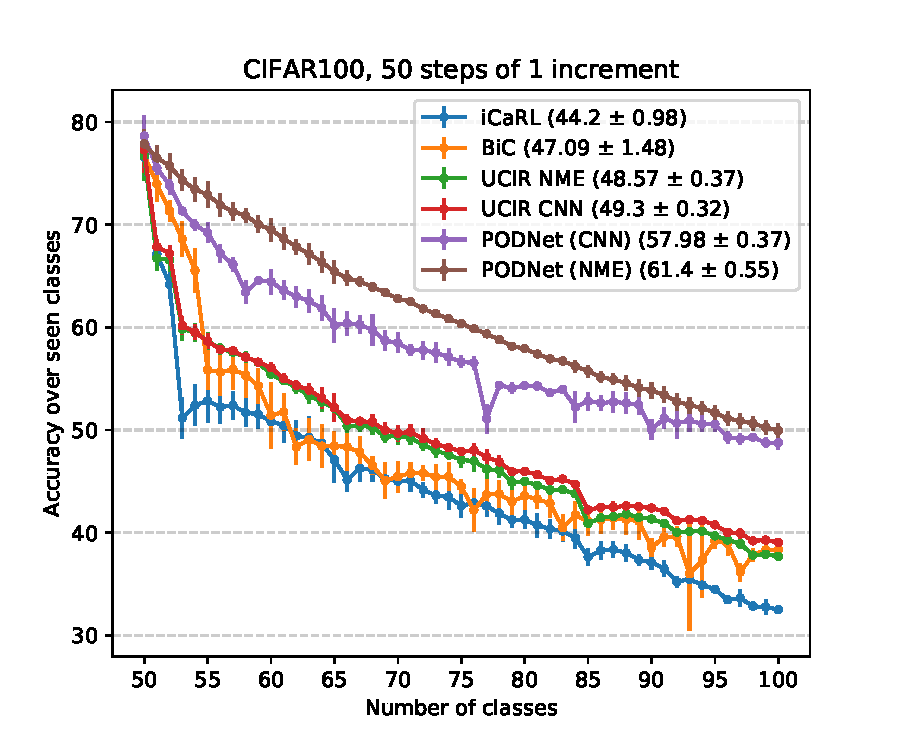
\includegraphics[width=\linewidth]{images/podnet/cifar_inc1}
        \caption{50 steps, 1 class / step}
        \label{fig:cifar_inc1}
    \end{subfigure}
    \hfill
    \begin{subfigure}[b]{0.48\linewidth}
        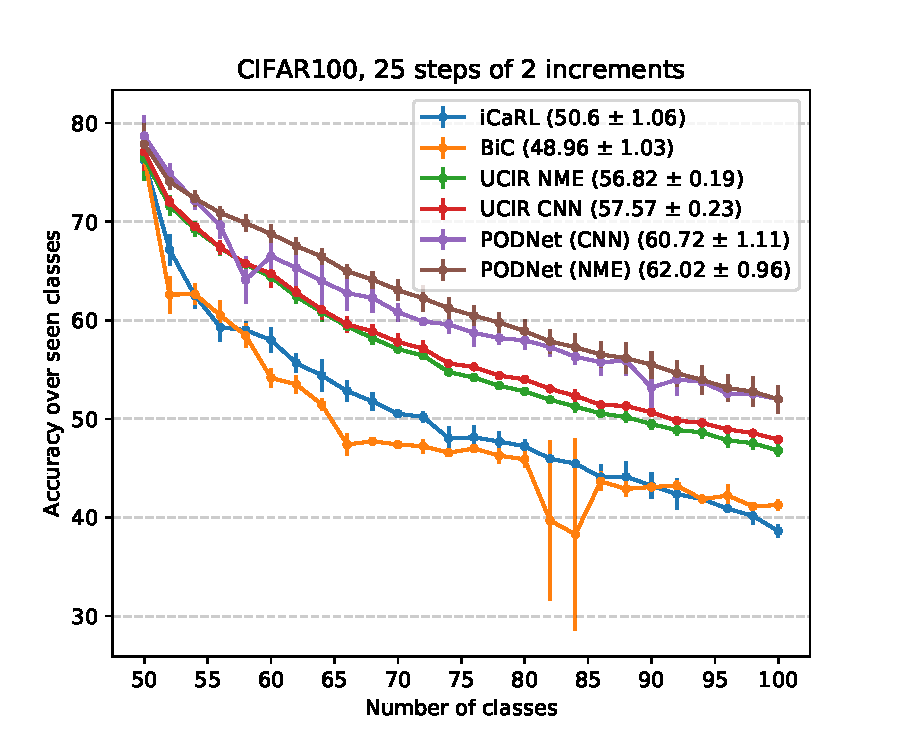
\includegraphics[width=\linewidth]{images/podnet/cifar_inc2}
        \caption{25 steps, 2 classes / step}
        \label{fig:cifar_inc2}
    \end{subfigure}
    \caption{\textbf{Incremental Accuracy on CIFAR100} over three orders for two different step sizes. The legend reports the average incremental accuracy.}
    \label{fig:plots}
\end{figure*}

\begin{table*}[t]
    \centering
    \begin{adjustbox}{max width=\textwidth}
        \begin{tabular}{@{}l|cccc|cc@{}}
            \toprule
                                                                             & \multicolumn{4}{|c|}{ImageNet100} & \multicolumn{2}{c}{Imagenet1000}                                                                                                         \\
            %\cmidrule(l{0pt}r{4pt}){2-4} \cmidrule(l{4pt}r{4pt}){5-7} \cmidrule(l{4pt}r{4pt}){8-9}
                                                                             & 50 steps                          & 25 steps                         & 10 steps                         & 5 steps                          & 10 steps       & 5 steps        \\
            \multicolumn{1}{r|}{New classes per step}                        & 1                                 & 2                                & 5                                & 10                               & 50             & 100            \\
            \midrule
            iCaRL* \scriptsize{\citep{rebuffi2017icarl}}                     & ---                               & ---                              & 59.53                            & 65.04                            & 46.72          & 51.36          \\
            iCaRL                                                            & 54.97                             & 54.56                            & 60.90                            & 65.56                            & ---            & ---            \\
            BiC \scriptsize{\citep{wu2019bias_correction}}                   & 46.49                             & 59.65                            & 65.14                            & 68.97                            & 44.31          & 45.72          \\
            UCIR\,{\scriptsize (\ac{NME})}* \scriptsize{\citep{hou2019ucir}} & ---                               & ---                              & 66.16                            & 68.43                            & 59.92          & 61.56          \\
            UCIR\,{\scriptsize (\ac{NME})}                                   & 55.44                             & 60.81                            & 65.83                            & 69.07                            & ---            & ---            \\
            UCIR\,{\scriptsize (CNN)}*                                       & ---                               & ---                              & 68.09                            & 70.47                            & 61.28          & 64.34          \\
            UCIR\,{\scriptsize (CNN)}                                        & 57.25                             & 62.94                            & 67.82                            & 71.04                            & ---            & ---            \\
            % PODNet\,{\scriptsize (CNN)}                & \textbf{62.48 $\pm$ 0.59} & \textbf{68.31 $\pm$ 2.45} & \textbf{74.33 $\pm$ 0.93} & \textbf{75.54 $\pm$ 0.26} & \textbf{64.13} & \textbf{66.95}\\
            PODNet\,{\scriptsize (CNN)}                                      & \textbf{62.48}                    & \textbf{68.31}                   & \textbf{74.33}                   & \textbf{75.54}                   & \textbf{64.13} & \textbf{66.95} \\

                                                                             & \scriptsize{\textbf{$\pm$ 0.59}}  & \scriptsize{\textbf{$\pm$ 2.45}} & \scriptsize{\textbf{$\pm$ 0.93}} & \scriptsize{\textbf{$\pm$ 0.26}} &                &                \\

            \bottomrule
        \end{tabular}
    \end{adjustbox}
    \caption{\textbf{ImageNet quantitative experiments:} Average incremental accuracy, PODNet \vs
        state of the art. Models with an asterisk * are reported directly from \citet{hou2019ucir}.
        The initial task's sizes are respectively 50 and 500 classes for ImageNet100 and
        ImageNet1000. The remaining classes are learned incrementally.}
    \label{tab:podnet_quantitative_imagenet}
\end{table*}



\subsubsection{Quantitative results}
\label{sec:podnet_quantitative_results}

The comparisons with all the State-of-the-Art are tabulated in
\autoref{tab:podnet_quantitative_cifar} for CIFAR100 and \autoref{tab:podnet_quantitative_imagenet}
for ImageNet100 and ImageNet1000. All tables show the average incremental accuracy for each
considered models with various number of steps on the incremental learning run. The ``New classes
per step'' row shows the amount of new classes introduced per task.

\paragraph{CIFAR100} We run our comparisons on 5, 10, 25, and 50 steps with respectively 10, 5, 2,
and 1 classes per step. We created three random class orders to run each experiment thrice,
reporting averages and standard deviations. For CIFAR100 only, we evaluated our model with two
different kinds of inference: \ac{NME} and CNN. With both methods, our model surpasses all previous
State-of-the-Art models on all steps. Moreover, our model relative improvement grows as the number
the steps increases, surpassing existing models by 0.82, 2.81, 5.14, and 12.1 percent points (\pp)
for respectively 5, 10, 25, and 50 steps. Larger numbers of steps imply  stronger forgetting; those
results confirm that PODNet manages to reduce drastically the said forgetting. While
PODNet with \ac{NME} has the largest gain, PODNet with CNN also outperforms the previous
State-of-the-Art by up to 8.68\pp. See \autoref{fig:podnet_plots} for a plot of the incremental
accuracies on this dataset. In the extreme setting of 50 increments of 1 class
(\autoref{fig:podnet_cifar_inc1}), our model showcases large differences, with slow degradation
(``\textit{gradual forgetting}'' \citep{french1999catastrophicforgetting}) due to forgetting
throughout the run, while the other models show a quick performance collapse (``\textit{catastrophic
    forgetting}'') at the start of the run.

\paragraph{ImageNet100} We run our comparisons on 5, 10, 25, and 50 steps with respectively 10, 5,
2, and 1 classes per step. For both ImageNet100, and ImageNet1000 we report only PODNet with
CNN, as the kNN-based \ac{NME} classifier did not generalize as well to larger-scale datasets. With
the more complex images of ImageNet100, our model also outperforms the State-of-the-Art on all
tested runs, by up to 6.51\pp.

\paragraph{ImageNet1000} This dataset is the most challenging, with much greater image complexity
than CIFAR100, and ten times the number of classes as ImageNet100. We evaluate the models in 5 and
10 steps, and results confirm the consistent improvement of PODNet against existing arts by up
to 2.85\pp.

\begin{table*}
    \centering
    \begin{tabular}{@{}lccccc@{}}
        \toprule
        Classifier & POD-flat & POD-spatial & NME            & CNN            \\
        \midrule
        Cosine     &          &             & 40.76          & 37.93          \\
        Cosine     & \OK      &             & 48.03          & 46.73          \\
        Cosine     &          & \OK         & 54.32          & 57.27          \\
        Cosine     & \OK      & \OK         & 56.69          & 55.72          \\
        LSC-CE     & \OK      & \OK         & 59.86          & 57.45          \\
        LSC        &          &             & 41.56          & 40.76          \\
        LSC        & \OK      &             & 53.29          & 52.98          \\
        LSC        &          & \OK         & \textbf{61.42} & 57.64          \\
        LSC        & \OK      & \OK         & 61.40          & \textbf{57.98} \\
        \bottomrule
    \end{tabular}
    \caption{Comparison of the average incremental accuracy on CIFAR100 with 50 steps of the model when disabling parts of the complete \ac{PODNet} loss\\~}
    \label{tab:podnet_ablation_inc}
\end{table*}


\subsubsection{Further analysis \& ablation studies}
\label{sec:podnet_ablation}

\paragraph{Ablation Studies}
Our model has two components: the distillation loss \ac{POD} and the \ac{LSC} classifier. An
ablation study showcasing the contribution of each component is displayed in
\autoref{tab:podnet_ablation_inc}: each additional component improves the model performance. We
evaluate every ablation on CIFAR100 with 50 steps of 1 new class each. The reported metric is the
average incremental accuracy. The table shows that our novel method of constraining the whole
\ac{ConvNet} is beneficial. Furthermore, applying only POD-spatial still beats the previous state of
the art by a significant margin. Using both POD-spatial and POD-flat then further increases results
with a large gain. We also compare the results with the Cosine
classifier~\citep{luo2018cosine_classifier,hou2019ucir} against the \acf{LSC} with NCA loss.
Finally, we add \ac{LSC}-CE: our classifier with multimode but with a simple cross-entropy loss
instead of our modified NCA loss. This version brings to mind SoftTriple~\citep{qian2019softtriple}
and Infinite Mixture Prototypes~\citep{allen2019infinitemixtureproto}, used in the different context
of few-shot learning. The latter only considers the closest mode of each class in its class
assignment, while \ac{LSC} considers all modes of a class, thus, taking into account the intra-class
variance. That allows \ac{LSC} to decrease class similarity when intra-class variance is high (which
could signal a lack of confidence in the class).

\begin{table*}
    \centering
    \begin{tabular}{@{}lcc@{}}
        \toprule
        Loss                                                        & NME            & CNN            \\
        \midrule
        \textit{None}                                               & 53.29          & 52.98          \\
        POD-pixels                                                  & 49.74          & 52.34          \\
        POD-channels                                                & 57.21          & 54.64          \\
        POD-gap                                                     & 58.80          & 55.95          \\
        POD-width                                                   & 60.92          & 57.51          \\
        POD-height                                                  & 60.64          & 57.50          \\
        POD-spatial                                                 & \textbf{61.40} & \textbf{57.98} \\
        \cmidrule{1-3}
        GradCam~\citep{dhar2019learning_without_memorizing_gradcam} & 54.13          & 52.48          \\
        Perceptual Style~\citep{johnson2016perceptual_losses}       & 51.01          & 52.25          \\
        \bottomrule
    \end{tabular}
    \caption{\textbf{Comparison of distillation losses} based on intermediary features. All losses evaluated
        with POD-flat. We report the average incremental accuracy on CIFAR100 with 50 steps.}
    \label{tab:podnet_ablation_perceptual}
\end{table*}



\label{sec:podnet_ablation_pooling}
\paragraph{Spatial-based distillation} We apply our distillation loss \ac{POD} differently for the
flat final embedding $\vh$ (POD-flat) and the \ac{ConvNet}'s intermediate features maps $\vh_\ell$
(POD-spatial). We designed and evaluated several alternatives for the latter whose results are shown
in \autoref{tab:podnet_ablation_perceptual}.
Refer to \autoref{sec:podnet_pod} for their definition. In this table, all losses are with
POD-flat ("\textit{None}" is using only POD-flat). Note that We provide in the appendix
(\autoref{sec:appendix_podnet}) the same table without POD-flat.

Overall, we see that not using pooling results in bad performance (POD-pixels). Our final loss,
POD-spatial, surpasses all others by taking advantages of the statistics aggregated from both
spatial axis. For the sake of completeness, we also included losses not designed by us: GradCam
distillation~\citep{dhar2019learning_without_memorizing_gradcam} and Perceptual
Style~\citep{johnson2016perceptual_losses}. The former uses a gradient-based attention while the
later --\,used for style transfer\,-- computes a gram matrix for each channel.

\paragraph{Forgetting and plasticity balance} Forgetting can be drastically reduced by imposing a
high factor on the distillation losses. Unfortunately, it will also degrade the capacity (its
\textit{plasticity}) to learn new classes. When POD-spatial is added on top of POD-flat
(\autoref{tab:podnet_ablation_perceptual}), we manage to increase the oldest classes' performance (+7
percentage points) while the newest classes' performance were barely reduced (-0.2\pp). Because our
loss POD-spatial constraints only statistics, it is less stringent than a loss based on exact pixels
values as POD-pixel. The latter hurts the newest classes (-2\pp) for a smaller improvement of old
classes (+5\pp). Furthermore, our experiments confirmed that \ac{LSC} reduced the sensibility of the
model to distribution shift, as the performance it brings was localized on the old classes.

\label{sec:podnet_robustness}
\paragraph{Robustness of our model} While previous results showed that PODNet improved
significantly over the state-of-the-arts, we wish here to demonstrate here the robustness of our
model to various factors. In \autoref{tab:podnet_ablation_memorysize}, we compared how PODNet
behaves against the baseline when the memory size per class $M_{\text{per}}$ changes: PODNet
improvements increase as the memory size decrease, up to a gain of 26.20\pp\ with \ac{NME} (resp.
13.42\pp\ for CNN) with $M_{\text{per}} = 5$. Notice in our main experiments
(\autoref{sec:podnet_quantitative_results}), only 20 images per class are kept in the memory. More
experiments validating our model's robustness are provided in the appendix
(\autoref{sec:appendix_podnet}).


\begin{table}[t]
    \centering
    \begin{tabular}{@{}lccccccc@{}}
        \toprule
        $M_{per}$                                                       & 5              & 10             & \textbf{20}    & 50             & 100            & 200            \\
        \midrule
        iCaRL \scriptsize{\citep{rebuffi2017icarl}}                     & 16.44          & 28.57          & 44.20          & 48.29          & 54.10          & 57.82          \\
        BiC \scriptsize{\citep{wu2019bias_correction}}                  & 20.84          & 21.97          & 47.09          & 55.01          & 62.23          & \textbf{67.47} \\
        UCIR\,{\scriptsize (\ac{NME})} \scriptsize{\citep{hou2019ucir}} & 21.81          & 41.92          & 48.57          & 56.09          & 60.31          & 64.24          \\
        UCIR\,{\scriptsize (CNN)}                                       & 22.17          & 42.70          & 49.30          & 57.02          & 61.37          & 65.99          \\
        PODNet\,{\scriptsize (\ac{NME})}                                & \textbf{48.37} & \textbf{57.20} & \textbf{61.40} & \textbf{62.27} & \textbf{63.14} & 63.63          \\
        PODNet\,{\scriptsize (CNN)}                                     & \textbf{35.59} & \textbf{48.54} & \textbf{57.98} & \textbf{63.69} & \textbf{66.48} & \textbf{67.62} \\
        \bottomrule
    \end{tabular}
    \caption{\textbf{Effect of the memory size} per class $M_{per}$ on the models performance.
        Results from CIFAR100 with 50 steps, we report the average incremental accuracy}
    \label{tab:podnet_ablation_memorysize}
\end{table}




\FloatBarrier

\section{Ghost: avoiding pre-emptively forgetting via ghost features}
\label{sec:ghost}

With PODNet, we reduced forgetting by reducing the shift of feature statistics between the old and
new model. Orthogonally, we also explored if we could regularize the intermediate latent space so
that forgetting could be avoided ---or at least reduced--- before even the introduction of
disrupting new classes. This idea draw inspiration from \cite{aljundi2019selfless} who remarked that
the ability to make room for future classes is a key limitation of current continual learning
models, and propose a regularization loss to make the model more “selfless”, by leaving capacity for
future classes in the representation. However, this pre-allocation of the future classes is done
without supervision by enforcing sparsity. We propose instead to pre-allocate explicitly using weak
information about the future classes. Drawing inspiration from the \acf{ZSL} literature
\citep{lampert2009zeroshot}, we exploit classes metadata to estimate the representation of future
classes.

\begin{comment}
Continual learning aims to perform equally well on past and present tasks. We proposed instead a
challenging new setting, \textit{prescient continual learning}, in which the model must perform well
not only for present and past tasks, but also for \textit{future} ones, both avoiding catastrophic
forgetting (using a limited number of training samples for past classes), and giving the best
possible estimates for the future classes (using no training samples at all). To make the setting
possible, the model must know the classes and have some prior information about them. Indeed,
\cite{aljundi2019selfless} remark that the ability to make room for future classes is a key
limitation of current continual learning models, and propose a regularization loss to make the model
more “selfless”, explicitly leaving capacity for future classes in the representation.
\cite{hanrebuffi2020autodiscovering} proposed a setting where the training samples from all classes
are present from the beginning, but the labels become available incrementally. In a way, our setting
is the inverse: we know which labels we will encounter, but the training data for those labels
arrive incrementally. For instance, in many real-world applications (\eg fashion product
classification), due to budget constraints, models are released incrementally, with partial classes
and training data, despite the classes being known from the beginning, and being well-characterized
by attributes.
\end{comment}

\subsection{Related Works}
\label{sec:ghost_related}

To address the proposed model, we take inspiration from \acf{ZSL}
\citep{lampert2009zeroshot,xian2019awa2}, which allows classifying examples from unseen classes by
combining a vision model with an embedding possessing knowledge about the classes (\eg a word
embedding \citep{mikolov2013word2vec,pennington2014glove} or an attribute matrix). Although several
approaches exist for zero-shot learning, we will focus on generating a representation for the future
classes \citep{bucher2017zeroshot_gmmn, kumar2018synthesized_zeroshot,
    xian2018feature_generating_zeroshot}. The framework of representation learning will allow us to
integrate continual and zero-shot learning seamlessly, as we advance through the tasks and future
classes become present classes, and then past classes. Moreover, we will be able to use
\textit{ghost features}, predicted features for the future classes, to make room in the
representation space for future classes. All those goals all integrated into a simple, streamlined
model due to a careful construction of the losses.

The contributions of this work are two-fold: (1) we propose a new challenging setting,
\textit{prescient} continual learning, where the model must perform well on past, present, and
\textit{future} classes; (2) we propose our \textit{ghost model} to address that setting,
integrating continual and zero-shot learning into a coherent whole where future classes are
pre-allocated, reducing their ---yet not happened--- forgetting.


\subsection{Setting: Prescient Continual Learning}
\label{sec:ghost_setting}

\begin{figure}
    \centering
    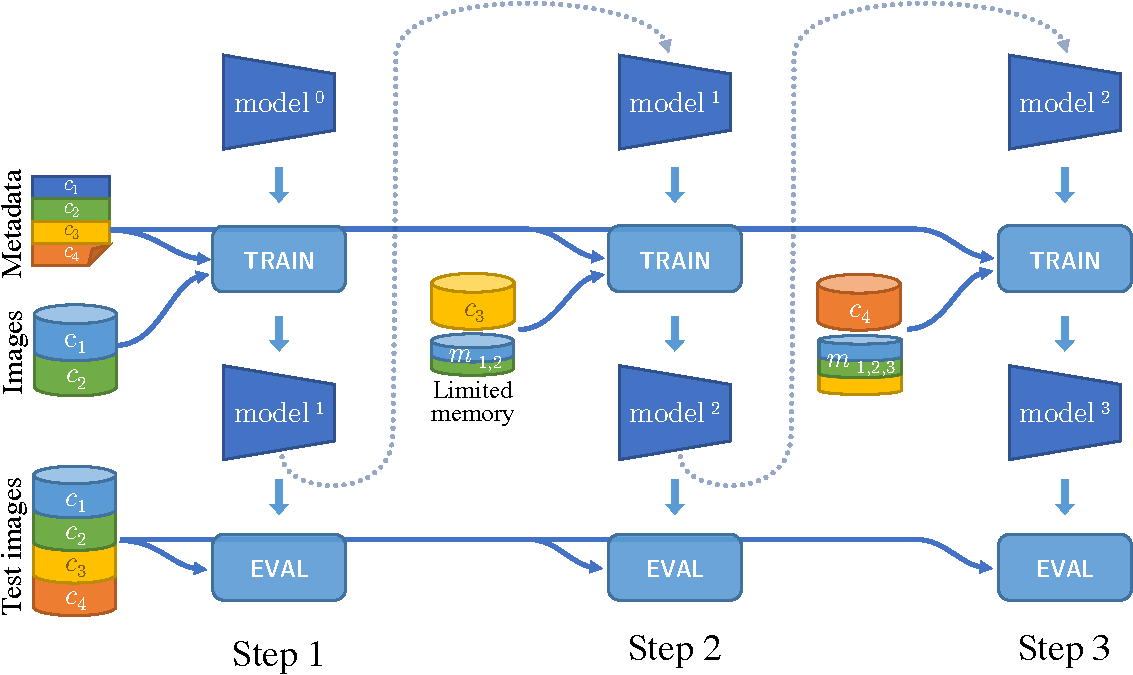
\includegraphics[width=0.7\linewidth]{images/ghost/protocol.pdf}
    \caption{\textbf{Prescient Continual Learning}. At each training task, we learn a new set of
        classes, but the model is evaluated on \textit{all classes} --- past, present, and future.
        The model has to avoid catastrophic forgetting of past classes (using a limited number of
        rehearsal training samples), as well as make a good guess for future classes (using no
        training samples at all).}
    \label{fig:ghost_protocol}
\end{figure}


We propose an enriched experimental setting, prescient continual learning, that extend the class
incremental setting used in \autoref{fig:podnet_model}, in which each task is evaluated on
\textit{all classes} $\mcC^{1:T}$: past ($\mcC^{1:t-1}$), present ($\mcC^t$), and future
($\mcC^{t+1:T}$). In that challenging new setting, we must not only avoid the catastrophic
forgetting of past classes (using the limited rehearsal training samples), but also give our best
estimates for future classes (using no training samples at all). That will only be possible if we
have some prior information about the classes, \eg their hierarchy in a semantic network (like
WordNet \citep{fellbaum1998wordnet}), an associated word embedding (like Word2Vec
\citep{mikolov2013word2vec}), or an attribute matrix. Such setting is illustrated in
\autoref{fig:ghost_protocol}. We will shorthand the set of past and present classes $\mcC^{1:t}$ as
the \textit{seen} classes, and the set of future classes $\mcC^{t+1:T}$ as the \textit{unseen}
classes. We denote individual samples by a superscript $\vx^(i)$, the class label by a subscript
$\vx_c$, and on which parameters a loss is applied by a subscript $\mcL_\Theta$.

\subsection{Model}
\label{sec:ghost_model}

To address the setting described in the previous section, we propose our \textit{ghost model},
comprising three components: a convolutional feature extractor $f$, a feature generator $g$, and a
classifier $\clf$. The feature extractor is the backbone of the model: it learns to extract a
feature vector from actual samples that can be fed to the classifier. The generator learns the
distribution of the features for all classes, aiming to generate plausible samples of features for
the future classes. The classifier makes the final decision for all classes: past, present, and
future. The classifier is trained on future classes with features sampled from the generator, which
we call \textit{ghost features} (since they must be “hallucinated” from the seen classes and some
prior knowledge about the classes).

The base model, on which Ghost is built, is either PODNet (detailed in \autoref{sec:podnet}) or UCIR
\citep{hou2019ucir}, both metric-based models.

\subsubsection{Capacitating ghost model for future classes}
\label{sec:ghost_zeroshot}

The base model can deal with both present classes (with training samples constrained only by their
availability in the training set)  and past classes (with training samples severely constrained by
the rehearsal memory). As discussed, the introduction of a distillation loss prevents catastrophic
forgetting of the latter. We will now address \textit{future classes}, with \textit{no} training
samples available. First, taking inspiration from zero-shot learning, we will use prior information
about the classes to generate \textit{ghost features}, plausible stand-ins for the unseen future
classes' features. Next, we will adapt the classifier to incorporate those ghost features into the
learning objective seamlessly. The representation learning framework will allow us to integrate the
entire learning apparatus into one coherent loss.

\paragraph{Generator} The generative model estimates the distribution of the unseen classes directly
in terms of their features (instead of the input images). For the feature generation to work, we
must have exploitable prior information about the classes, more precisely, we must be able to map
the class labels $c$ into a \textit{class attribute space} that makes semantic sense. The exact way
to perform that mapping will be data-dependent, but most often, either we will have an explicit set
of attributes linked to each class (color, size, material, provenance, etc.), or we will be able to
extract a latent semantic vector, using a technique like Word2vec
\citep{mikolov2013word2vec,pennington2014glove}. The generator learns to link the attributes of the
\textit{seen} classes to the actual feature vectors extracted from the training samples of those
classes. Thus, the first generator training must happen after the feature extractor (its
ground-truth) is learned. The generator is fine-tuned after each task to handle distribution shift.
Next, we ask the generator to draw random samples, using the attributes of the \textit{unseen}
classes, creating counterfeit features that we call \textit{ghost features}. The strategy is
agnostic to the generator model as long as it can be conditioned by class attributes.  At present,
as detailed in \autoref{sec:ghost_quantitative}, we choose a Generative Moment Matching Network
\citep{li2015gmmn}: a shallow multi-layer perceptron conditioned by class attributes and a noise
vector trained to minimize the Maximum Mean Discrepancy
\citep{gretton2007twosampleMMD,gretton2012twosampletestMMD} between the estimated features
$\tilde{\vh}^t_c$ and the actual features $\vh^t_c$ for each class $c$ among the current classes
$\mcC^t$, produced by the feature extractor $f$.

\begin{figure}
    \centering
    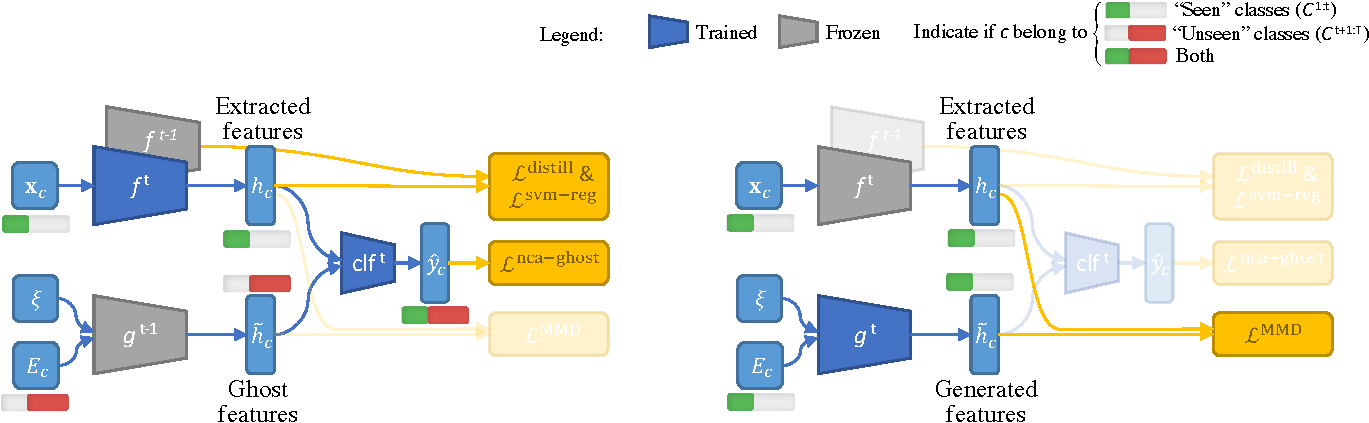
\includegraphics[width=\linewidth]{images/ghost/model.pdf}
    \begin{subfigure}{.5\textwidth}
        \vspace{2mm}
        \centering
        \caption{Training of the classifier}
        \label{fig:ghost_training_cls}
    \end{subfigure}%
    \begin{subfigure}{.5\textwidth}
        \vspace{2mm}
        \centering
        \caption{Training of the generator}
        \label{fig:ghost_training_gen}
    \end{subfigure}
    \caption{\textbf{Procedure to train our model applied at each task/step}: (a) a complete classifier is learned with seen and unseen features ($\mcL^\text{\tiny{nca-ghost}}$). The feature extractor is protected from catastrophic forgetting ($\mcL^\text{\tiny{distill}}$), and constrained to separate seen classes from unseen/ghosts classes ($\mcL^\text{\tiny{svm-reg}}$). (b) Once a task is done, the generator is fine-tuned on the new latent space ($\mcL^\text{\tiny{MMD}}$) on seen classes. Notice that for the first and last tasks, the classifier does not use the ghost features.}
    \label{fig:ghost_training_procedure}
\end{figure}


\label{sec:ghost_generator}

\paragraph{Complete classifier} Remind that the parameters  $\{\theta_c\,,\forall c \in \mcC^{1:t}\}$ on
the representation-based classifier (\autoref{eq:podnet_lsc}) may be interpreted as proxies for the
classes $\mcC^{1:t}$. The base model for task $t$ will, thus, learn $\mcN^{1:t} = |\mcC^{1:t}|$ such
proxies, one for each of the seen classes. To extend the model for the unseen future classes, the
complete classifier will learn $\mcN^{1:t} + \mcN^{t+1:T}$ proxies, which changes
\autoref{eq:podnet_nca} to:
%
\begin{equation}
    \mcL^\text{\tiny{nca-ghost}}_{\Theta_f,\Theta_{\clf}} = \left[- \log\frac{\exp\left(\vyh_y - \delta\right)}{\sum_{\substack{c \neq y\\c \in \mcC^{1:t}}} \exp \vyh_{c} + \sum_{\substack{c \neq y\\c \in \mcC^{t+1:T}}} \exp \vyh_{c}} \right]_+ \,.
    \label{eq:ghost_nca}
\end{equation}
%
This classification loss maximizes the similarity $\vyh_y$ (or, conversely, minimizes the distance)
between sample feature $\vh_y$ and correct class proxy $\theta_y$ in the numerator. In the denominator,
the loss pushes away all wrong class proxies, from both seen and unseen (future) classes, by
minimizing the similarities with $\vy_c, \, \forall c \neq y$.

The participation of future classes in the classification loss has two effects. Most obviously, it
allows the model to perform zero-shot-like guesses for those classes during test time. The
representation-learning paradigm allows performing both continual and zero-shot learning seamlessly,
as we advance through the tasks and future classes become present classes, and then past classes.
Less evidently, but vitally important, the learning of proxies for the future classes makes room in
the representation space for those classes, creating effective empty spaces that push away the
actual features of the seen classes (due to the repulsive term in the denominator). As we advance
through training, future classes become present, their ghost placeholders disappear, and they can
neatly fit in the newly vacant region. Such a strategy reduces interference between classes
throughout continual learning, and, as we will see in both visual and quantitative experiments, has
long-range positive effects.

Naturally, the complete classifier has to be trained with samples from all classes. For seen
classes, actual data is available from the training and rehearsal data. For unseen future classes
data is not available, so we employ ghost features sampled from the generator. Note that ghost
features are produced once per task by the generator and are kept fixed for the task duration.
\label{sec:ghost_classifier}

\begin{figure}
    \centering
    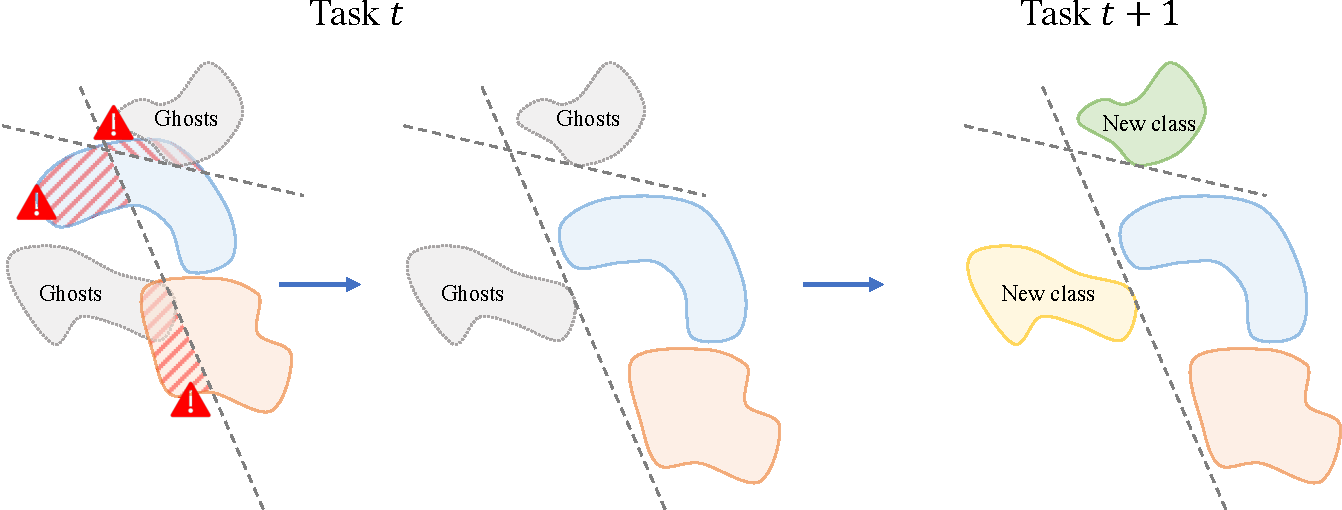
\includegraphics[width=0.7\linewidth]{images/ghost/svm_reg.pdf}
    \caption{\textbf{Latent-space regularization} establishes margin-based one-unseen-class \vs
        all-seen-classes linear separations. Those separations are employed to directly condition the
        feature space, creating space for future unseen classes. In the following task, some unseen
        classes will become seen, and may occupy the feature space with less interference.}
    \label{fig:ghost_svm_reg}
\end{figure}

\label{sec:ghost_svm}
\paragraph{Latent-space regularization}
As explained above, our Ghost classification loss minimizes the intra-class distances and maximizes
the inter-class distances. The loss enforces those constraints to all proxies regardless of whether
they represent seen classes or not. We further promote an inter-class separation by optimizing the
latent representation of seen classes to avoid overlapping with the representation of Ghosts. That
loss constrains the features space directly and does not affect the proxies and the intra-class
distances.

We based this regularization loss on SVM \citep{cortes1995svm} for simplicity, but other methods
could have similar behavior. To compute that loss, we learn binary
one-unseen-class-Vs-all-seen-classes SVM classifiers, one for each unseen class. We employ a linear
kernel, since the feature extractor and feature vector dimensionality (512) allows good linear
separation, but more complex kernels could be used. Those \acs{SVM} define hyperplanes
$\mathbf{w}_c$ and biases $b_c,\, \forall c \in \mcC^{t+1:T}$, separating each unseen region from the
mass of seen features $\mathbf{h}^{(i)}$ (\autoref{fig:ghost_svm_reg}):
%
\begin{equation}
    \mcL^\text{\tiny{svm-reg}}_{\Theta_f} = \frac{1}{\mcN^{t+1:T}} \sum_{c\in \mcC^{t+1:T}} [\mathbf{w}_c \cdot \vh^t + b_c + \tau]_+\,,
    \label{eq:ghost_svm}
\end{equation}
%
\noindent where $\vh^t$ are seen features (classes in $\mcC^{1:t}$), $[\,\cdot\,]_+$ the hinge loss,
and $\tau$ an additional margin (higher values of $\tau$ push seen features further away from the
ghost regions, in practice, we set $\tau=1$ to repel beyond the support vectors).

The margin-based regularization of \autoref{eq:ghost_svm} refines the ghost classification loss of
\autoref{eq:ghost_nca}. While the latter acts over the classifier conditioning the feature space
indirectly via the action of the class proxies, the former acts directly over the latent/feature
space and the feature extractor backbone that creates it. The computational overhead of training
several SVMs, detailed in the appendix (\autoref{sec:appendix_ghost}), is negligible compared to the total training
time.

\paragraph{Complete strategy} All modules and losses fit neatly into the goal of learning
continuously over seen and unseen classes. We train feature extractor (plus classifier) and
generator in alternation. We train the latter to mimic the features of seen classes, and then ask it
to extrapolate to unseen classes (ghost features). Ghost features allow us both to unify seen and
unseen classes into a complete classifier ($\mcL^\text{\tiny{nca-ghost}}$), and to enforce early
allocation in the feature space for unseen classes ($\mcL^\text{\tiny{svm-reg}}$). The complete
loss, in addition to a distillation loss to counter-act catastrophic forgetting
($\mcL^\text{\tiny{distill}}$), is:
%
\begin{equation}
    \mcL = \mcL^\text{\tiny{nca-ghost}}_{\Theta_f,\Theta_{\clf}} + \lambda_1 \mcL^\text{\tiny{distill}}_{\Theta_f} + \lambda_2 \mcL^\text{\tiny{svm-reg}}_{\Theta_f}\,.
    \label{eq:ghost_loss}
\end{equation}
%
The model is illustrated in \autoref{fig:ghost_training_procedure} and \autoref{algo:ghost_task_training} is the
algorithm of our model in pseudocode, showcasing a procedural view of the execution of one task.

\begin{algorithm}[H]
    \begin{algorithmic}[1]
        \Require
        \Statex task id $t$
        \Statex $f^t$, $c^t$, and $g^t$
        \Statex Data from new task and rehearsal memory $(X, y)$

        \If{$t = 1$ or $t = T$} \State Train $f^t$ and $g^t$ with $\mcL^\text{\tiny{nca}}$
        and $\mcL^\text{\tiny{distill}}$ on $(\vx, y)$ and Ghost samples. \Else \State Train $f^t$ and $g^t$
        with $\mcL^\text{\tiny{nca-ghost}}$, $\mcL^\text{\tiny{svm-reg}}$ and $\mcL^\text{\tiny{distill}}$
        on $(\vx, y)$ and Ghost samples. \EndIf

        \State Evaluate on all classes: $\mcC^{1:t} \cup \mcC^{t+1:T}$.

        \If{$t \ne 1$ and $t < T - 1$} \State Train $g^t$ with $\mcL^\text{\tiny{MMD}}$ using attributes of
        seen classes $\mathbf{E}_{c} \,, \forall c \in \mcC^{1:t}$ \State Generate Ghost samples for next
        task using attributes of unseen classes $\mathbf{E}_{c} \,, \forall c \in \mcC^{t+2:T}$ \EndIf
    \end{algorithmic}
    \caption{Task procedure of the Ghost model}
    \label{algo:ghost_task_training}
\end{algorithm}


\subsection{Experiment Results}
\label{sec:ghost_exp}

\subsubsection{Pictorial experiments}
\label{sec:ghost_pictorial}

Before running our full-scale experiments, we perform a set of experiments with a model that keeps
the main components from the proposed model in a simplified form that will allow us to link
quantitative performances to intuitive visual plots of the feature spaces. For the experiments in
this section we employ the MNIST \citep{lecun2010mnist} dataset, with an initial task of 6 classes
(digits 0 to 5), then two more tasks of two classes each; the feature extractor comprises two
convolutional layers followed by a fully connected layer outputting a feature vector of only two
dimensions — a purposeful choice to allow easy visualization of the feature space. Because MNIST
classes have no attributes, we cannot apply zero-shot learning directly. Instead, we employ the
features of actual images from the future classes instead of samples from the generator — which
corresponds, in some ways, to have a perfectly calibrated generator. Those features are extracted
once per task, and the feature extractor is never trained on unseen classes images. As we will see
in \autoref{tab:ghost_generated_vs_real}, integrating the generator in our full-scale model
outperforms using actual extracted features, so that necessary substitution does not exaggerate the
abilities of this small-scale model. The losses used to train the small and the full-scale models
are the same, but the SVM-based regularization was not employed since it made little sense for a 2D
latent space.

The 2D feature space allows us to directly visualize the evolution of the feature space as the tasks
progress, without the need for dimensionality reduction techniques that complicate the analysis
(\eg t-SNE \citep{maaten2008tsne}). \autoref{fig:ghost_toy_weights_3steps} may be interpreted
upfront: as the three tasks progress left-to-right, we see the evolution of the feature space on the
base model (PODNet, on the top branch) and on the proposed model with ghost features (bottom
branch). The base model presents a strong overlap between the initial classes, and the latter added  8
({\color{orange}orange}) and 9 ({\color{violet}dark purple}). That comes partially from shape
similarities (‘8’ is similar to ‘0’ and ‘5’), partially from continual learning, and results in
severe forgetting of old classes in favor of new ones. The proposed model organizes better the
feature space, which is particularly visible between the second and third steps, where the early
allocation of ghost zones for the future classes (displayed as empty black circles) is prominent.
That better arrangement of the feature space increases the final accuracy from 44 to 66\%, a 22 \pp
improvement. The small latent space of 2 dimensions explains the low performance for both models; a
model that learns on all classes in one step (\textit{i.e.} not in a continual setting) reaches only
69\% of final accuracy. That said, our model shows a clear improvement both qualitatively in
\autoref{fig:ghost_toy_weights_3steps} and quantitatively. More experiments of this kind can be
found in the appendix (\autoref{sec:appendix_ghost}).

\begin{figure}
    \centering
    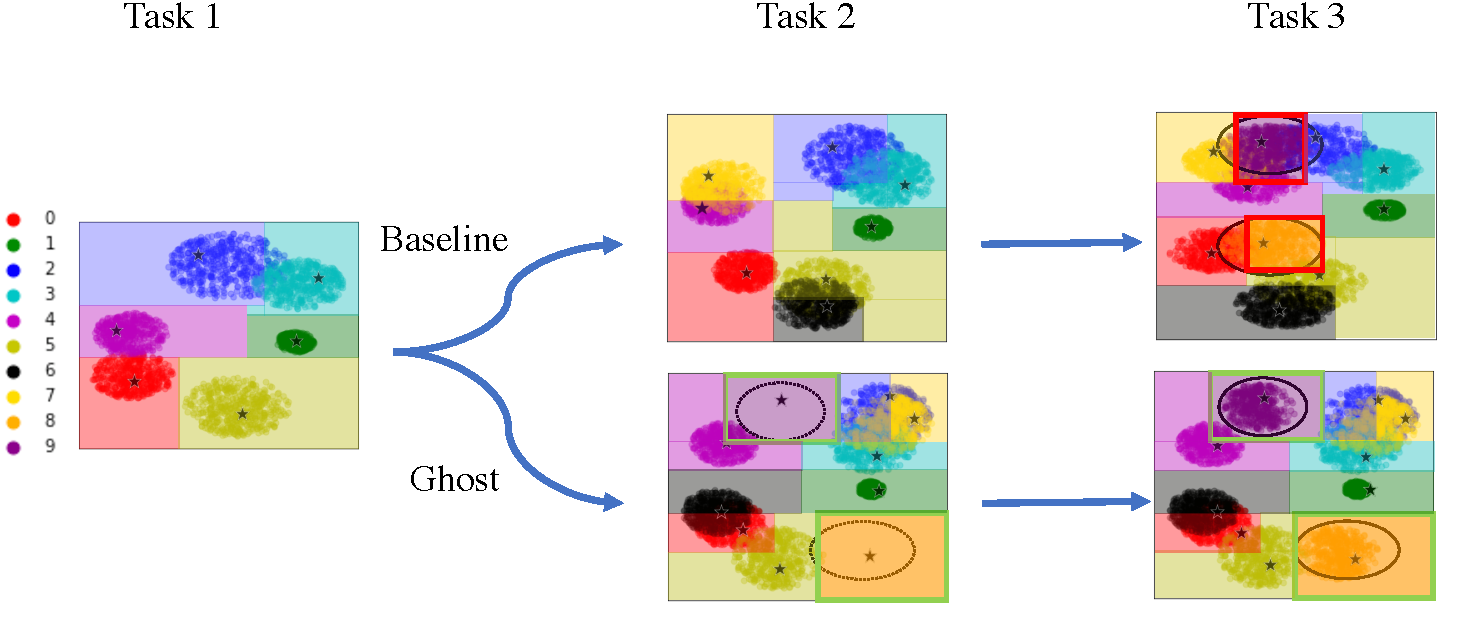
\includegraphics[width=0.8\linewidth]{images/ghost/toy_model_6_2_2.pdf}
    \caption{\textbf{Small-scale PODNet} on MNIST with 3 steps (digits '0' to '5'; then '6' and '7';
        then '8' and '9') with a features space of only two dimensions. The early incorporation of
        ghost features/proxies in the second task, denoted by dotted circles in the bottom row,
        enforces vacant space for those unseen classes. When filled in the third task (last column),
        there is less interference/overlap with previous classes. Such a strategy improves the final
        accuracy by 22 \pp.}
    \label{fig:ghost_toy_weights_3steps}
\end{figure}

\subsubsection{Main experiments}
\label{sec:ghost_quantitative}

\paragraph{Datasets \& Protocols} We perform our experiments on two datasets: AwA2
\cite{xian2019awa2}, with 50 animals categories, each with 85 attributes; and AP\&Y
\cite{farhadi2009apy}, with 32 everyday object classes, each with 64 attributes. We employ two
experimental protocols: one typical for continual learning, following
\cite{hou2019ucir,douillard2020podnet}, starting the first task with half the classes (i.e., 25 for
AwA2, and 16 for aP\&Y), then adding the remaining classes in evenly-sized tasks (5 tasks of 5
classes for AwA2, and 8 tasks of 2 classes for aP\&Y); another inspired from zero-shot learning,
following \cite{xian2019awa2}, starting with a standard selection of classes for each of the
datasets (40 for AwA2, and 20 for aP\&Y), and adding the remaining classes in small increments (5
tasks of 2 classes for AwA2, and 6 tasks of 2 classes for aP\&Y). Our evaluation protocol is akin to
the challenging and realist Generalized Zero-shot Learning \citep{scheirer2013generalizedzeroshot,
    chao2016generalizedzeroshot} protocol with no information on whether a sample is from a seen or
unseen class — but harsher, since classes are seen gradually, and training samples for past classes
data are limited by rehearsal memory.

\paragraph{Base Models} We evaluate our contributions on top of two different representation-based
models, both based on ResNet18 \citep{he2016resnet} feature extractor backbones (with feature vector
size of 512) and cosine classifiers. They differ on the distillation loss $\mcL_\text{distil}$
employed, the first model (PODNet)
constraining the statistics of the intermediate features after each residual block (\autoref{sec:podnet}), and the second
(UCIR) using Hou et al.'s distillation \citep{hou2019ucir} enforcing a cosine constraint on the
final flat latent space. The former performs better than the latter, but both are improved by the
innovations proposed in this work. The cosine classifier has a single proxy/representative per class
but could easily be generalized to multiple proxies. Implementation details are provided in the
appendix (\autoref{sec:appendix_ghost}).

\paragraph{Generator} Following the work of \cite{bucher2017zeroshot_gmmn} for zero-shot
learning, our generator is a Generative Moment Matching Network (GMMN)~\cite{li2015gmmn}
$g^t(\mathbf{\xi}, \mathbf{E}_c)$, which takes as inputs a Gaussian noise vector $\mathbf{\xi}$ and
a class attributes vector $\mathbf{E}_c$, and outputs a sample from the estimated distribution of
features for a class with the given attributes. In our experiments on AwA2 and AP\&Y, the class
attributes vectors are the average of the attributes for the training samples in the class. For each
task $t$, the feature extractor $f^t$ and the generator $g^t$ are trained to minimize the Maximum
Mean Discrepancy (MMD) \citep{gretton2007twosampleMMD,gretton2012twosampletestMMD} between the
actual features of seen classes $\vh_c = f^t(\vx_c) \, , \forall c \in \mcC^{1:t}$ and their
distribution on the generator $\tilde{\vh}_c = g^t(\mathbf{\xi}, \mathbf{E}_{c}) \,, \forall c \in
    \mcC^{1:t}$.

We train the generator and the main model (feature extractor and classifier) alternately, as shown
in \autoref{fig:ghost_training_procedure}. We always train the generator at the end of the task,
after the feature extractor has adapted to the new distribution (\autoref{fig:ghost_training_gen}).
Then, we use the generator to produce ghost samples for the next task (unless we have reached the
last task, with no unseen classes) which are fed to the feature extractor
(\autoref{fig:ghost_training_cls}).

When training the generator, we first extract features for all seen classes, with free access to the
training samples for the present classes, but only a limited number (given by the rehearsal memory)
for the past classes. For better numerical behavior, we scale each dimension of the extracted
features to the interval [0, 1] before feeding them to the generator (and then re-scale the output
of the generator back to the original intervals before feeding its samples to the classifier). The
generator is trained to minimize the Maximum Mean Discrepancy (MMD) between the features of seen
concepts $\vh_c = f^t(\vx_c) \, , \forall c \in \mcC^{1:t}$ and the representation it generates
$\tilde{\vh}_c = g^t(\mathbf{\xi}, \mathbf{E}_{c}) \,, \forall c \in \mcC^{1:t}$:
%
\begin{equation}
    \mcL^\text{\tiny{MMD}}_{\Theta_g} = \left\Vert \frac{1}{N} \sum_{i=1}^N \phi\big(\vh^{(i)}_c\big) - \frac{1}{N} \sum_{j=1}^N \phi\big(\tilde{\vh}^{(j)}_c\big) \right\Vert^2\,, \quad c \in \mcC^{1:t}\,,
    \label{eq:mmd_loss}
\end{equation}
%
\noindent with $\phi(\cdot)$ being a Gaussian kernel, and the superscript $\cdot^i$ denotes the
$i^{th}$ sample. The trained generator uses the attributes of the classes
— which is the only information we have about them — to estimate sample features that we call
\textit{ghost features}. To better estimate the statistics, we use all the real features of a single
seen class per batch. We denote the number of real features by $N$. The generator produces as many
ghost features as real features.

Our main model has mechanisms to fight Catastrophic Forgetting, which we found were sufficient also
to protect the generator. The feature extractor has an explicit distillation loss to prevent the
problem, and since its output is used to train the generator, the latter is also protected.
We considered applying a distillation loss to the generator, trying to minimize a drift between
the produced features of the previous and current generator. We measured such drift according to
several metrics: cosine similarity, Kullback-Leiber divergence, L2 distance, and maximum mean
discrepancy. The first metric, cosine similarity, gave the best results. However, as the generator was
well protected, we gained at most 0.50 Continual Accuracy \pp on AwA2.


\begin{table*}
    \caption{Continual Accuracy on AwA2 and aP\&Y for PODNet and UCIR.}
    \label{tab:continual_half}
    \centering
    \begin{tabular}{@{}l|cc|cc@{}}
        \toprule
                                                                                    & \multicolumn{2}{c}{AwA2}                              & \multicolumn{2}{c}{aP\&Y}                                                                                           \\
                                                                                    & \multicolumn{2}{c}{25 classes + 5 $\times$ 5 classes} & \multicolumn{2}{c}{16 classes + 8 $\times$ 2 classes}                                                               \\
                                                                                    & PODNet \cite{douillard2020podnet}                     & UCIR \cite{hou2019ucir}                               & PODNet \cite{douillard2020podnet} & UCIR \cite{hou2019ucir} \\
        \midrule
        Baseline                                                                    & 62.92 \std 0.12                                       & 54.80 \std 0.40                                       & 58.64 \std 0.66                   & 43.42 \std 0.21         \\
        \tableindent+ $\mcL^\text{\tiny{nca-ghost}}$                                & 68.31 \std 0.36                                       & 57.88 \std 0.27                                       & 62.08 \std 0.25                   & 50.23 \std 0.29         \\
        \tableindent+ $\mcL^\text{\tiny{nca-ghost}}$ + $\mcL^\text{\tiny{svm-reg}}$ & 68.46 \std 0.47                                       & 58.08 \std 0.46                                       & 62.73 \std 0.60                   & 50.91 \std 0.56         \\
        %\tableindent+ $\mcL_\text{svm-reg}$ & 63.34 \std 0.13 & 55.34 \std 0.28 & \tbd &\tbd \\
        \bottomrule
    \end{tabular}
\end{table*}

\begin{table*}
    \caption{Final Accuracy on AwA2 and aP\&Y for PODNet and UCIR.}
    \label{tab:final_half}
    \centering
    \begin{tabular}{@{}l|cc|cc@{}}
        \toprule
                                                                                    & \multicolumn{2}{c}{AwA2}                              & \multicolumn{2}{c}{aP\&Y}                                                                                           \\
                                                                                    & \multicolumn{2}{c}{25 classes + 5 $\times$ 5 classes} & \multicolumn{2}{c}{16 classes + 8 $\times$ 2 classes}                                                               \\
                                                                                    & PODNet \cite{douillard2020podnet}                     & UCIR \cite{hou2019ucir}                               & PODNet \cite{douillard2020podnet} & UCIR \cite{hou2019ucir} \\
        \midrule
        Baseline                                                                    & 77.63 \std 0.06                                       & 67.07 \std 0.81                                       & 57.80 \std 0.97                   & 42.23 \std 1.34         \\
        \tableindent+ $\mcL^\text{\tiny{nca-ghost}}$                                & 78.70 \std 0.46                                       & 67.43 \std 0.08                                       & 62.47 \std 0.40                   & 44.17 \std 1.48         \\
        \tableindent+ $\mcL^\text{\tiny{nca-ghost}}$ + $\mcL^\text{\tiny{svm-reg}}$ & 79.08 \std 0.53                                       & 67.53 \std 0.45                                       & 63.30 \std 0.98                   & 45.97 \std 0.26         \\
        %\tableindent+ $\mcL_\text{svm-reg}$ & 78.50 \std 0.10 & 67.0 \std 0.17 & \tbd & \tbd \\
        \bottomrule
    \end{tabular}
\end{table*}


\paragraph{Continual Learning with Future Classes}
For continual learning, it is usual to take into account the model's performance as it evolves. We
adapt the traditional average incremental accuracy \citep{rebuffi2017icarl}
(\autoref{eq:related_avg_acc} in \autoref{sec:related_metrics}) to take into account \textit{all}
classes, including the future ones, and call that metric \textit{continual accuracy}: the average of
accuracy over all seen classes after each task. The results appear in
\autoref{tab:ghost_continual_half}, which shows, for the datasets and protocols explained in the top
of this section, the performance for our two base models \citep{hou2019ucir,douillard2020podnet},
and the improvements on those base models as we implement our proposed model, with and without the
SVM latent-space regularization refinement. The ability to guess a future class' representation
brings large improvements on both datasets, for both base models. The SVM-based regularization
refinement also improves the results, by up to 0.65 \pp.

\begin{figure}
    \centering
    \begin{subfigure}{0.45\linewidth}
        \centering
        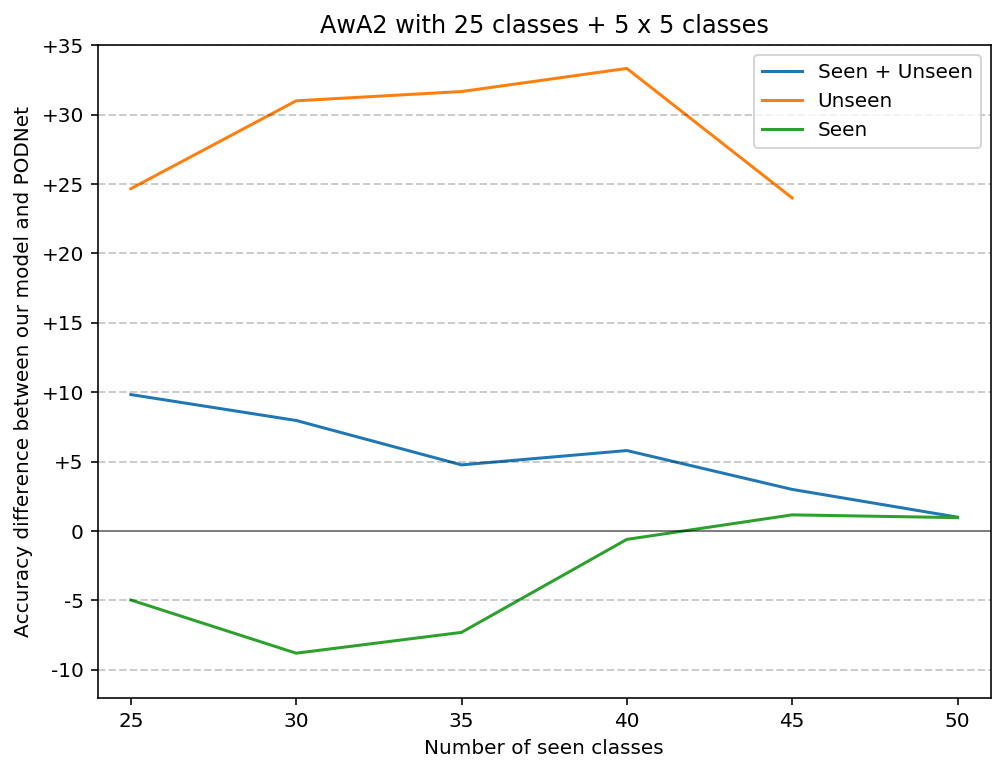
\includegraphics[width=\linewidth]{images/ghost/plot_awa2_25x5x5c_podnet_diff.png}
        \caption{Ghost vs PODNet.}
    \end{subfigure}
    \begin{subfigure}{0.45\linewidth}
        \centering
        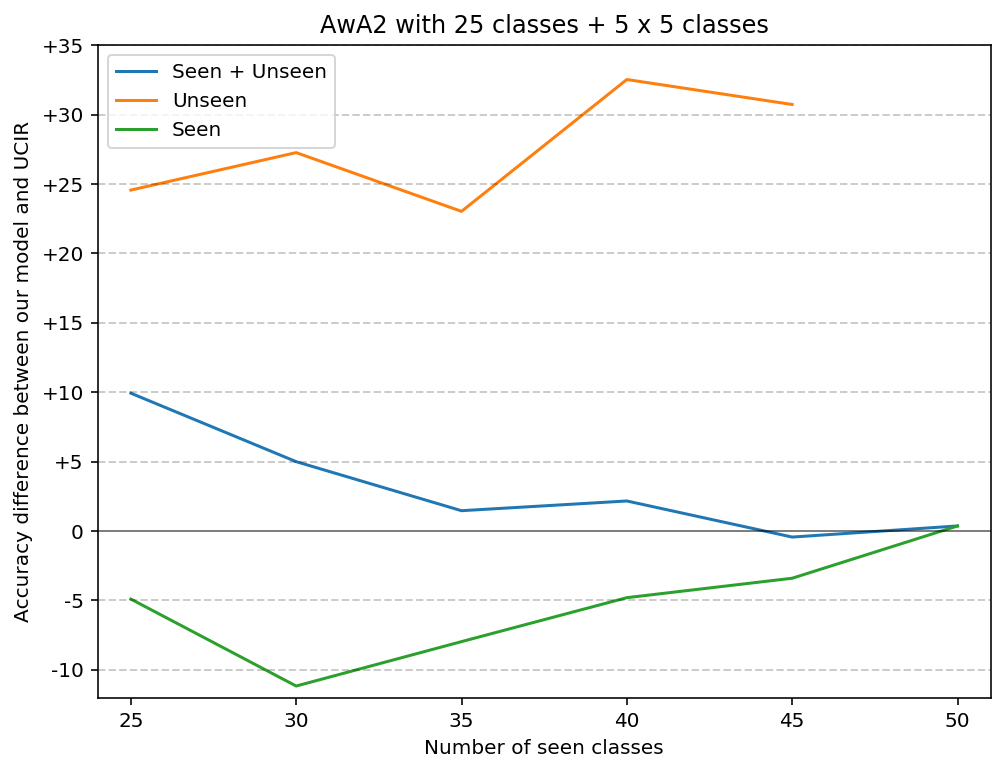
\includegraphics[width=\linewidth]{images/ghost/plot_awa2_25x5x5c_ucir_diff.png}
        \caption{Ghost vs UCIR}
    \end{subfigure}
    \caption{\textbf{Difference of accuracy} over all classes, only seen classes, and only unseen
        classes Ghost model vs base models on AwA2.}
    \label{fig:ghost_plot_awa2_25x5x5c}
\end{figure}


\paragraph{Final Accuracy} Once we reach the final task, the proposed model ability to guess future
classes provides no advantage due to all classes being now seen. Still, as shown in
\autoref{tab:ghost_final_half} — where the metric is simply the accuracy at the final task of each
run (\autoref{eq:related_final_acc} in \autoref{sec:related_metrics}) — the proposed method
outperforms the baselines, due to a better organization of the feature space. Although the numerical
advantages in this table are smaller than in the previous one, these results are consequential,
showing that the ability of the proposed model of incorporating knowledge about the classes is
useful beyond the zero-shot scenario. Again, the SVM-regularization refinement helps by up to 1.80
\pp.

\paragraph{Model Evolution} To showcase how the models evolve, plots contrasting the proposed
methods with each base model (PODNet and UCIR) task by task appear in
\autoref{fig:ghost_plot_awa2_25x5x5c}. The plots show how, on early tasks, the main advantage of the
proposed model is its ability to guess on the future classes, while on the final task no future
classes remain, but the proposed model still keeps a (more modest, but definitive) advantage.

\begin{table}
    \caption{Further experiments where the initial task size correspond to standard zero-shot seen classes \cite{xian2019awa2}. We report Continual and Final Accuracies for PODNet on AwA2 and aP\&Y.}
    \label{tab:initial_seen}
    \centering
    \begin{tabular}{@{}l|cc|cc@{}}
        \toprule
                                                                                    & \multicolumn{2}{c}{AwA2}                              & \multicolumn{2}{c}{aP\&Y}                                                                 \\
                                                                                    & \multicolumn{2}{c}{40 classes + 5 $\times$ 2 classes} & \multicolumn{2}{c}{20 classes + 6 $\times$ 2 classes}                                     \\

                                                                                    & Continual                                             & Final                                                 & Continual       & Final           \\
        \midrule
        PODNet \cite{douillard2020podnet}                                           & 82.84 $\pm$ 0.10                                      & 84.70 $\pm$ 0.10                                      & 67.57 \std 0.41 & 65.23 \std 0.50 \\
        \tableindent+ $\mcL^\text{\tiny{nca-ghost}}$                                & 84.99 $\pm$ 0.17                                      & 86.57 $\pm$ 0.49                                      & 68.80 \std 0.98 & 67.93 \std 1.24 \\
        \tableindent+ $\mcL^\text{\tiny{nca-ghost}}$ + $\mcL^\text{\tiny{svm-reg}}$ & 84.47 \std 0.15                                       & 85.73 \std 0.40                                       & 69.02 \std 0.46 & 67.97 \std 0.60 \\
        %\tableindent+ $\mcL_\text{svm-reg}$ & 83.58 \std 0.12 & 85.70 \std 0.2° & \tbd & \tbd\\
        \bottomrule
    \end{tabular}
\end{table}


\paragraph{Zero-shot-like Initial Task Setting} This set of experiments
(\autoref{tab:ghost_initial_seen}) is intended for comparison with zero-shot learning benchmarks
\citep{xian2019awa2}, which always use the same split of seen/unseen classes for a given dataset.
Our first task in the continual learning contains the classes defined in zero-shot benchmark as
seen, and we learn next, in small increment, the remaining classes, i.e., those defined in the
zero-shot benchmark as unseen. Because the initial task is larger than previously, fewer future
classes remain, and the base models have better performance. Still, the proposed method improves
both base methods in both datasets significantly. The setting proposed is different from the —
markedly less challenging — setting appearing in \cite{pkankuekul2012onlineincrementalzeroshot} and
\cite{xue2017incrementalzeroshot}, where the set of unseen classes is fixed, and only more seen
classes are added incrementally, without any sample limitations given by rehearsal memory.


\begin{table*}
    \centering
    \begin{adjustbox}{max width=\textwidth}
        \begin{tabular}{@{}l|cc|cc@{}}
            \toprule
                                          & \multicolumn{2}{c}{AwA2}                              & \multicolumn{2}{c}{aP\&Y }                                                                              \\
                                          & \multicolumn{2}{c}{25 classes + 5 $\times$ 5 classes} & \multicolumn{2}{c}{16 classes + 8 $\times$ 2 classes}                                                   \\
                                          & Continual                                             & Final                                                 & Continual              & Final                  \\
            \midrule
            %\textit{None} & &  & \OK & 62.92 \std 0.12 & 77.63 \std 0.06 & 58.64 \std 0.66 & 57.80 \std 0.97\\
            Our model                     & 68.46 \std 0.47                                       & 79.08 \std 0.53                                       & 62.73 \std 0.60        & 63.30 \std 0.98        \\
            \tableindent w/ real features & 67.65 \std 0.50                                       & 78.83 \std 0.31                                       & 61.88 \std 0.52        & 61.70 \std 0.26        \\
            \gray{Partial oracle}         & \gray{72.94 \std 0.25}                                & \gray{84.60 \std 0.28}                                & \gray{63.81 \std 0.29} & \gray{68.03 \std 1.42} \\
            \gray{Full oracle}            & ---                                                   & \gray{95.40 \std 0.02}                                & ---                    & \gray{97.40 \std 0.30} \\
            \bottomrule
        \end{tabular}
    \end{adjustbox}
    \caption{\textbf{Comparison of generated ghost features vs. actual features} extracted from future classes'\,samples with PODNet on AwA2 and aP\&Y.}
    \label{tab:ghost_generated_vs_real}
\end{table*}


\paragraph{Generator Validation} The generator approximates the feature extractor for the unseen
future classes. To validate its effectiveness, we replace the generated features with the actual
features from the future images. This form of “cheating”, of course, is not possible in
\textit{actual} real-world scenarios, but serves as a metric. \autoref{tab:ghost_generated_vs_real}
shows the comparison, with the surprising result that generated features performed better than the
actual features from samples (respectively first and second row). Note that the latter are extracted
once per task. We hypothesize it explains the score difference because the feature extractor was
never adapted for the unseen classes distribution. The "oracle" experiments in the third and fourth
row in \autoref{tab:ghost_generated_vs_real} establish an upper bound for what we could achieve by
"cheating" around the experimental protocol restrictions. The partial oracle from third row is the
same model as the second row, fine-tuning the feature extractor with samples coming from the future.
The full oracle of the fourth line uses all images from all classes without any restriction in a
single task. Despite the partial oracle has full access to real future data, we stress that our
model's performance with generated future data is close to this upper bound.


\begin{figure}[httb!]
    \centering
    \begin{subfigure}{.45\textwidth}
        \centering
        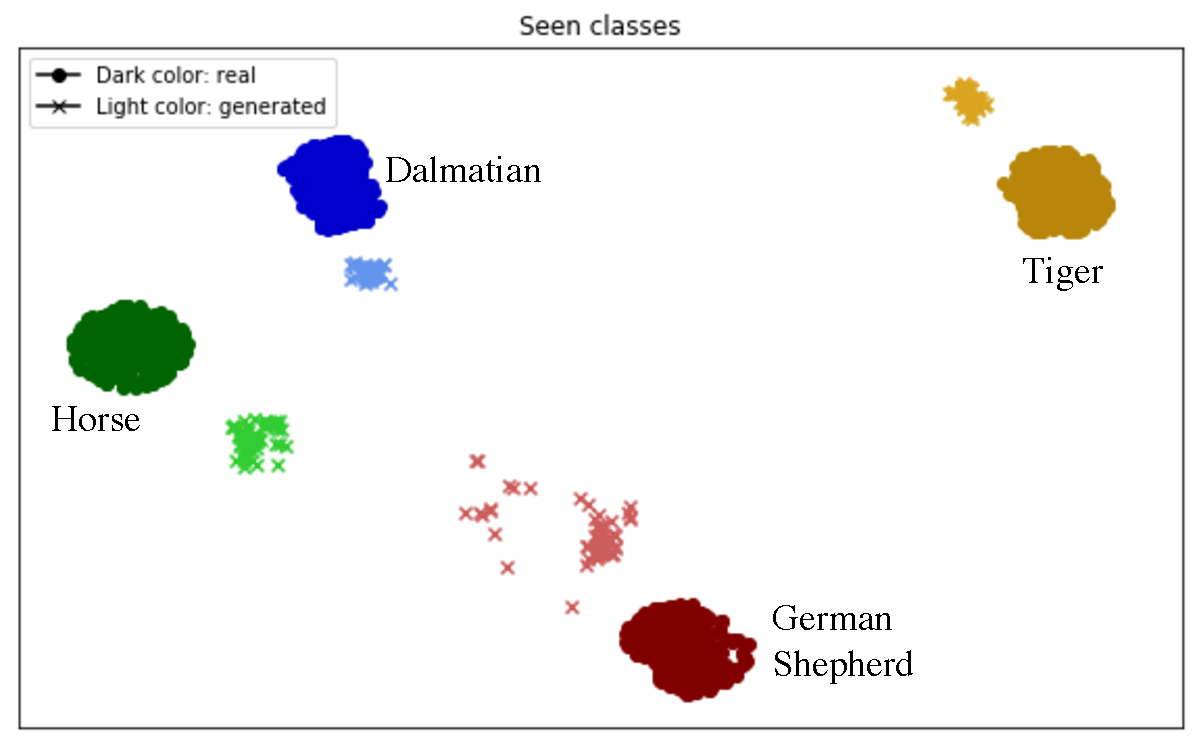
\includegraphics[width=\linewidth]{images/ghost/tsne_seen.pdf}
        \caption{Generator interpolation for \textit{seen} classes.}
        \label{fig:ghost_tsne_seen}
    \end{subfigure}%
    \hspace{1em}
    \begin{subfigure}{.45\textwidth}
        \centering
        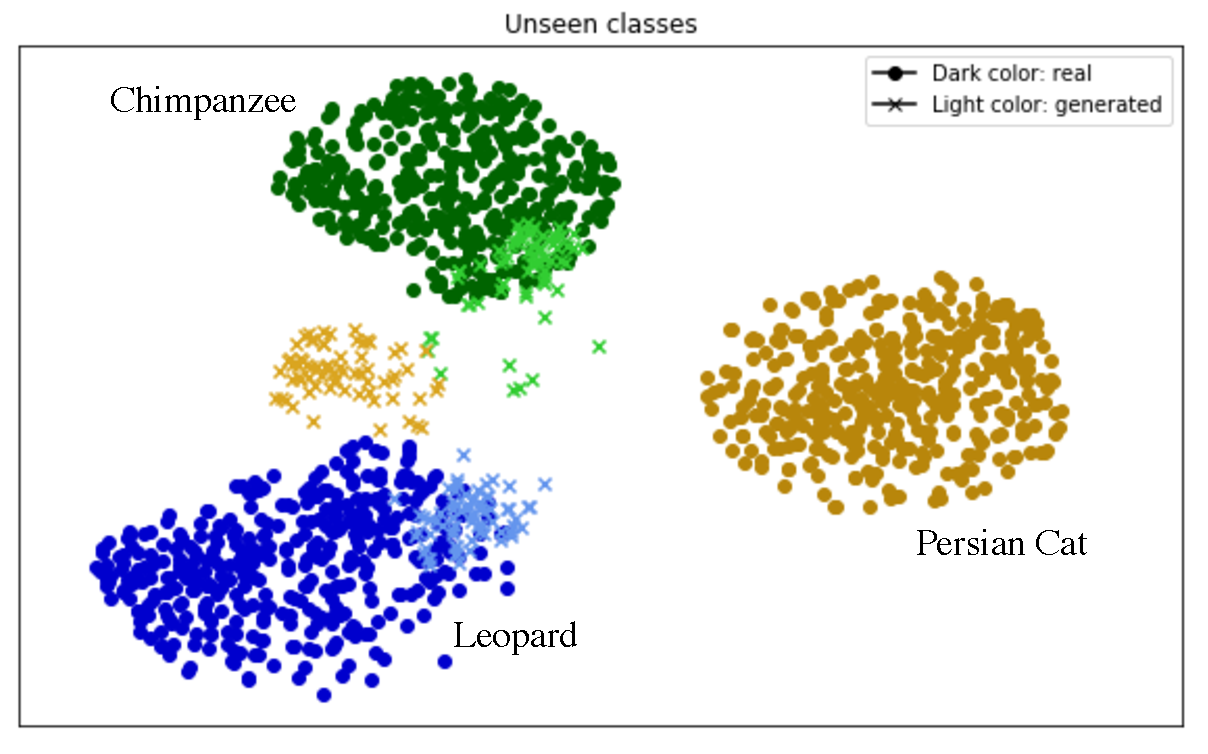
\includegraphics[width=\linewidth]{images/ghost/tsne_unseen.pdf}
        \caption{Generator extrapolation for \textit{unseen} classes.}
        \label{fig:ghost_tsne_unseen}
    \end{subfigure}
    \caption{\textbf{t-SNE of the latent space}. Dark colors indicate real features, while lighter colors denote their generated homologous. Real features extracted with $f^t$, and ghost features sampled from $g^t$. Generation in (a) is both well-located and tightly bound because the GMMN was trained to approximate those seen classes. In (b), the generator is asked to extrapolate to unseen classes only from their attributes, resulting in more spread features — still surprisingly, in general, well-located. Notice that the even the real features in (b) gets more spread, since the feature extractor was never trained on those classes.}
    \label{fig:ghost_tsne}
\end{figure}


\paragraph{Ghost visualization} We inspect the ghost samples created by our generator with
visualization in \autoref{fig:ghost_tsne}: we compare the features extracted from the
actual images with their generated homologous, produced by the GMMN on the AwA2 dataset. To allow
visualization, we reduce the dimensionality of the features to two with t-SNE. In
\autoref{fig:ghost_tsne_seen}, we compare, at task $t$, the actual features (in dark colors) to generated
features (in light colors) for seen classes. The generated features are, in most cases, near the
clusters of real features, and all clusters — real and generated are tightly bound. We then compare
in \autoref{fig:ghost_tsne_unseen} the real and generated features on unseen classes. Compared to
\autoref{fig:ghost_tsne_seen}, even the real features show a bigger spread, due, we believe, to the
feature extractor $f^t$ not having met those unseen images. The generated features are also more
spread but are still, in general, reasonably placed, indicating the ability of the generator to
extrapolate — at least partially — the features for unseen classes from their attributes.

\section{Conclusion}

In this chapter, We covered our works on regularizations of the feature space. We proposed to
regularize, not the model's outputs as the vast majority of the literature, but intermediate
features. In this context, we tackle catastrophic forgetting via two approaches. Those approaches
are orthogonal and can be combined.

The first approach, PODNet, reduces the drift between the old and new models by constraining
statistics of the intermediate features. We show that a naive constraint balances poorly the
plasticity-rigidity trade-off. Thus, we propose carefully designed pooling to directly exploit the
spatial nature of the images. By constraining long-range statistics of the horizontal and vertical
axes, we reduce drastically forgetting, especially in challenging settings with a large number of
tasks with few classes per task. Furthermore, we design a robust metric-based classifier that
exploits the multi-modality of the classes.

The second approach, Ghost, avoids pre-emptively forgetting by estimating the future locations of
yet unseen classes. Drawing inspiration from the zeroshot Learning literature, we exploit present classes'
metadata to generate what we called "Ghost features" of the future classes. We then regularize
the latent space, via a modified NCA loss and a SVM-based constraint, to allocate the future
locations of unseen classes. In addition, of the novel zeroshot capabilities, useful to the new
Prescient Continual Learning setting we introduced, we show that final performance has been improved
by avoiding confusion thanks to our pre-allocation strategy.
